% !TEX root = ../main_lecture_notes.tex
\chapter{Marche aléatoire et Martingale à temps discret}\label{chap:marche_aléatoire}
Ce cours propose une introduction au calcul stochastique avec pour application principale la modèlisation des marchés financiers et la gestion des risque en assurance. L'objet d'étude principale sont les processus stochastiques. 
\begin{definition}\label{def:filtration}
Soit $(\Omega, \F, \Prob)$ un espace probabilisé. Une suite $(X_t)_{t\geq0}$ de variable aléatoires (\va) sur $\Omega$ est un processus stochastique.
  \begin{itemize}
    \item Si $n\in \N$ alors $(X_n)_{n\geq0}$ est un processus stochastique à temps discret. Par exemple une chaine de Markov. 
    \item si $t\in \RL_+$ alors $(X_t)_{t\geq0}$ est un processus stochastique à temps continu. Par exemple le processus de Poisson. 
  \end{itemize}
\end{definition}
% L'utilisation des processus stochastiques pour comprendre le comportements des actifs financiers date des travaux de Bachelier. Près de 70 ans plus tard, Samuelson (prix nobel d'économie en 1970) proposa l'utilisation du mouvement Brownien avec drift. La théorie moderne repose sur les modèles de Black, Scholes and Merton, ce qu'on appelle la théorie des options et les arguments d'absence d'opportunité d'arbitrage. 
% \section{La marche aléatoire et le problème de la double dépense}
% \subsection{Blockchain, cryptomonnaie et double dépense}
% Une blockchain est une base de données constituée de blocs successifs maintenue par un réseau pair-à-pair, comme sur la \cref{fig:blockchain_network}. 
% \begin{figure}[ht!]
% \begin{center}
% \begin{tikzpicture}[-, >=, auto, semithick, node distance=01cm]
% \tikzstyle{every edge}=[segment length=1mm,segment angle=10, draw]

% \tikzstyle{full node}=[circle, fill=blue,draw=blue,thick,text=black,scale=0.8]
% \tikzstyle{light node}=[circle, fill=white,draw=blue,thick,text=black,scale=0.8]
% \node[full node]    (1)                     {};
% \node[full node]    (2)[above right of=1]         {};
% \node[full node]    (3)[above left of=1]         {};
% \node[full node]    (4)[below of=1]         {};
% \node[full node]    (5)[right of=4]         {};
% \node[full node]    (6)[below of=4]         {};
% \node[light node]    (7)[left of=1]         {};
% \node[light node]    (8)[right of=2]         {};
% \node[light node]    (9)[left of=4]         {};
% \node[light node]    (10)[above right of=5]         {};
% \node[light node]    (11)[ right of=5]         {};
% \node[light node]    (12)[ below right of=5]         {};
% % \node[light node]    (4)[above of=2]         {};
% \path

% (1) edge node{} (2)
%     edge node{} (3)
%     edge node{} (7)
%     ;
% \path
% (5) edge node{} (10)
%     edge node{} (11)
%     edge node{} (12)
%     ;
%     \path
% (4) edge node{} (5)
%     edge node{} (1)
%     edge node{} (9)
%     edge node{} (6)
%     ;
%     \path
% (2) edge node{} (8)   
%     ;
% \end{tikzpicture}
% \end{center}
% \caption{Un réseau fait de noeuds lourds (bleu) et de noeuds légers (blanc)}
% \label{fig:blockchain_network}
% \end{figure}
% Les noeuds légers se contentent d'émettre des informations (appelées transactions). Les noeuds lourds doivent vérifier la cohérence des transactions et s'accorder sur les informations à inscrire dans la blockchain. Les noeuds lourds appliquent un protocole de consensus pour se mettre d'accord. La preuve de travail ou \textit{Proof-of-Work} est le protocole utilisé dans le cadre de la blockchain des bitcoins, voir le whitepaper de \citet{Nakamoto2008}. Un bloc doit être ajouté toutes les dix minutes environ, les noeuds sont en compétition pour résoudre un problème cryptographique brutalement via une méthode essai-erreur (\textit{trial and error}). Le premier qui parvient à résoudre le problème ajoute le bloc et récupère une récompense d'un montant de BTC$6.25$ à l'heure de l'écriture.\footnote{\url{https://bitcoinblockhalf.com/}}. \\

% Dans la blockchain des bitcoins, les informations enregistrées sont des échanges de bitcoin entre les participants. Un noeud peut facilement émettre deux transactions conflictuelles, c'est à dire qui transfèrent les mêmes unités à deux entités différentes. Il s'agit d'une attaque par double dépense. Le scénario standard est le suivant:
% \begin{enumerate}
%     \item Marie transfère à John BTC$10$
%     \item La transaction de Marie à John est enregistrée dans la blockchain
%     \item John doit atendre $\alpha\in\N$ confirmations, c'est à dire que $\alpha$ blocs soient ajoutés après celui dans lequel la transaction de Marie à John est inscrite
%     \item Une fois que $\alpha$ confirmations ont été envoyées, John envoie le bien à Marie
%     \item Pendant ce temps, Marie travaille sur sa propre version de la blockchain (dite privée) dans laquelle la transaction de Marie à John est remplacée par une transaction de Marie à elle même
%     \item Au moment de la livraison du bien la blockchain dite principale est en avance de $z$ blocs 
%     \item L'objectif de Marie est générer une chaine concurrente plus longue que la chaine principale. Si elle y parvient, elle la communiquera à l'ensemble du réseau pour créer une fourche (\textit{fork}). Le réseau optera alors pour la branche la plus longue.
%     La branche de Marie va alors remplacer la branche principale permettant à Marie de récupérer ses unités qu'elle peut dépenser à nouveau. 
% \end{enumerate}
% Cette course entre les deux branches est résumée sur la \cref{fig:dp_illustration}.
% \begin{figure}[ht!]
% \begin{center}
% \begin{tikzpicture}[-, >=stealth', auto, semithick, node distance=1cm]
% % \tikzstyle{block} = [rectangle, draw, fill=blue!20,
% %     text width=5em, text centered, rounded corners]
% \tikzstyle{block}=[rectangle, fill=black,draw=black,thick,text=black,scale=1.5]
% \tikzstyle{block}=[rectangle, fill=white,draw=black,thick,text=black,scale=1.5]
% \tikzstyle{confirmed block}=[rectangle, fill=white,draw=blue,thick,text=black,scale=1.5]
% \tikzstyle{bad block}=[rectangle, fill=white,draw=red,thick,text=black,scale=1.5]
% \node[block]    (1)                     {\tiny $\text{M}\rightarrow \text{J}$};
% \node[block]    (2)[right of=1]                     {};
% \node[block]    (3)[right of=2]                     {};
% \node[block]    (4)[right of=3]                     {};
% \node[confirmed block]    (5)[right of=4]                     {};

% \node[bad block]    (6)[below of=1]         {\tiny $\text{M}\rightarrow \text{M}$};
% \node[block]    (7)[right of=6]         {};
% \node[block]    (8)[right of=7]         {};
% \path
% (1) edge[ left]     node{}     (2)
% (2) edge[ left]     node{}     (3)
% (3) edge[ left]     node{}     (4)
% (4) edge[ left]     node{}     (5)
% (6) edge[ left]     node{}     (7)
% (7) edge[ left]     node{}     (8);

% \end{tikzpicture}
% \end{center}
% \caption{La course à la double dépense illustrée, ici nous avons $\alpha = 4$ et $z = 2$}
% \label{fig:dp_illustration}
% \end{figure}
% Notre objectif est de caluler la probabilité que la branche de Marie devienne majoritaire. Pour ce faire nous allons construire un modèle mathématique.
\section{Le problème de ruine du parieur}
Un joueur entre dans un casino pour jouer à la roulette. Nous supposons que notre parieur dispose de $x\in \mathbb{N}$  jetons. Pour faire une partie, le joueur mise $1$ jetons. Il gagne $1$ jetons (et récupère sa mise) avec une probabilité $p\in(0,1)$ et perd sa mise avec probabilité $q = 1-p$.
\subsection{La marche aléatoire sur $\Z$}
Soit $(Z_n)_{n\in\mathbb{N}}$ le nombre de jetons de notre parieur après $n$ parties. On a $Z_0 = z\geq 0$. A chaque instant $k\in\N$ une partie est jouée, 
\begin{itemize}
    \item la partie est gagnée avec probabilité $p\in(0,1)$ et la réserve de jeton augment de $1$
    \item la partie est perdue avec probabilité $q = 1-p$ et la réserve diminue de $1$
\end{itemize}
Soit $(\Omega,\F, \Prob)$ un espace probabilisé. On définit une suite $(\xi_n)_{n\geq0}$ \iid de variables aléatoires (\va) de loi 
$$
\mathbb{P}(\xi = 1) = p\text{, et }\mathbb{P}(\xi = -1) = 1-p.
$$
On en déduit que 
$$
Z_n = z +\sum_{k=1}^n\xi_k.
$$ 
Le processus $Z_n$ est un processus à temps discret et à valeur dans $\Z$ appelé marche ou promenade aléatoire. Le parieur décide de s'arrêter de jouer si sa réserve de jetons atteint le niveau $a$ ou s'il est à cours de jeton. On définit les instants aléatoires
\begin{equation}\label{eq:dp_time}
\tau_0 = \inf\{n\geq0\text{ ; }Z_n = 0\},\text{ et }\tau_a = \inf\{n\geq0\text{ ; }Z_n = a\}.
\end{equation}
Nous souhaitons calculer la probabilité que le parieur rentre chez lui ruiné, c'est à dire 
\begin{equation}\label{eq:ruin_proba}
\phi(z, a) = \Prob(\tau_0 <\tau_a| Z_0 = z).
\end{equation}
Une visualisation du problème de première excursion est donné sur la \cref{fig:ruin_time}.
\begin{figure}[ht!]
\begin{center}
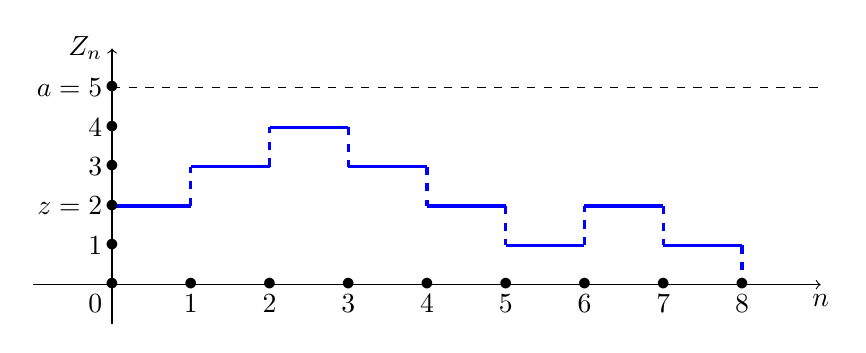
\begin{tikzpicture}
  %Origin and axis
  \coordinate (O) at (0,0);
  \draw[->] (-1,0) -- (9,0) coordinate[label = {below:$n$}] (xmax);
  \draw[->] (0,-0.5) -- (0,3) coordinate[label = {left:$Z_n$}] (ymax);
  \draw[dashed, -] (0,2.5) -- (9,2.5) coordinate[] (xmax);
  %Lower linear boundary

 
  %Stochastic process trajectory
  
  \draw (0,0) node[blue,left] {} node{};
  \draw[very thick,blue,-] (0,1) -- (1,1) node[pos=0.5, above] {} ;
  \draw[very thick,dashed,blue] (1,1) -- (1,1.5) node[pos=0.5, right] {};
  \draw[very thick,blue,-] (1,1.5) -- (2,1.5) node[pos=0.5, above] {};
  \draw[very thick,dashed,blue] (2,1.5) -- (2,2) node[pos=0.5, right] {};
  \draw[very thick,blue,-] (2,2) -- (3,2) node[pos=0.5, above] {};
  \draw[very thick,dashed,blue] (3,2) -- (3,1.5) node[pos=0.5, right] {};
  \draw[very thick,blue,-] (3,1.5) -- (4,1.5)node[pos=0.5, above] {};
  \draw[very thick,dashed,blue] (4,1.5) -- (4,1) node[pos=0.5, right] {};  
  \draw[very thick,blue,-] (4,1) -- (5,1) node[pos=0.5, above] {};
  \draw[very thick,dashed,blue] (5,1) -- (5,0.5) node[pos=0.5, right] {};  
  \draw[very thick,blue,-] (5,0.5) -- (6,0.5) node[pos=0.5, above] {};
  \draw[very thick,dashed,blue,-] (6,0.5) -- (6,1) node[pos=0.5, above] {};
   \draw[very thick,blue,-] (6,1) -- (7,1) node[pos=0.5, above] {};
    \draw[very thick,dashed,blue,-] (7,1) -- (7,0.5) node[pos=0.5, above] {};
     \draw[very thick,blue,-] (7,0.5) -- (8,0.5) node[pos=0.5, above] {};
     \draw[very thick,dashed,blue,-] (8,0.5) -- (8,0) node[pos=0.5, above] {};
  %Jump Times
  \draw (1,0) node[black,below] {$1$} node{ \color{black}$\bullet$};
  \draw (2,0) node[black,below] {$2$} node{ \color{black}$\bullet$};
  \draw (3,0) node[black,below] {$3$} node{ \color{black}$\bullet$};
  \draw (4,0) node[black,below] {$4$} node{ \color{black}$\bullet$};
  \draw (5,0) node[black,below] {$5$} node{ \color{black}$\bullet$};
  \draw (6,0) node[black,below] {$6$} node{ \color{black}$\bullet$};
  \draw (7,0) node[black,below] {$7$} node{ \color{black}$\bullet$};
  \draw (8,0) node[black,below] {$8$} node{ \color{black}$\bullet$};
  %Level of the counting process
   \draw (0,0) node[black,below left] {$0$} node{ \color{black}$\bullet$};
   \draw (0,0.5) node[black,left] {$1$} node{ \color{black}$\bullet$};
   \draw (0,1) node[black,left] {$z=2$} node{ \color{black}$\bullet$};
   \draw (0,1.5) node[black,left] {$3$} node{ \color{black}$\bullet$};
   \draw (0,2) node[black,left] {$4$} node{ \color{black}$\bullet$};
   \draw (0,2.5) node[black,left] {$a=5$} node{ \color{black}$\bullet$};

  % %Aggregated Capital gains
%  \draw (0,1.5) node[blue,below right] {$\mu_1$} node{ \color{blue}$-$};
%  \draw (0,2.25) node[blue,left] {$\mu_2$} node{ \color{blue}$-$};
%  \draw (0,3.75) node[blue,left] {$\mu_3$} node{ \color{blue}$-$};
  %Ruin time = First-crossing time time
%  \draw (5,0) node[black,above right] {${\tau_0}_u$} node{ \color{black}$\times$};
%  \draw[dotted,black] (0,3.28) -- (5,3.28);
%  \draw[dotted,black] (5,0) -- (5,3.28);
\end{tikzpicture}
\end{center}
\caption{Illustration du problème de premier passage sous-jacent à la double dépense.}
\label{fig:ruin_time}
\end{figure}

Le processus $Z$ est une chaine de Markov.
\subsection{Filtration, chaine de Markov et temps d'arrêt}
Soit $(\Omega,\F, \Prob)$ un espace probabilisé sur lequel on définit un processus $X:=(X_n)_{n\geq0}$. 
\begin{definition}\label{def:filtration}
Une filtration $(\F_n)_{n\geq0}$ est une suite de sous-tribu de $\F$, croissante pour l'inclusion au sens où
$$
\F_k\subset \F_n,\text{ pour }k\leq n.
$$

\end{definition}
$\F_n$ correspond à l'information disponible au temps $n$. C'est aussi l'information nécessaire pour tracer la trajectoire du processus jusqu'à l'instant $n$.
\begin{definition}\label{def:processus_adapte}
Le processus X est $\F_n$-adapté si $X_n$ est mesurable par rapport $\F_n$. La suite
$$
\F_n = \sigma(X_1,\ldots, X_n),\text{ }n\in \N,
$$ 
est la filtration naturelle du processus $X$.
\end{definition}
\begin{ex}\label{ex:filtration_marche_aleatoire}
La marche aléatoire $Z_n$ est adaptée à la filtration $$
\F_n = \sigma(\xi_k,\text{ }k\leq n).
$$
\end{ex}
Soit un processus $X:=(X_n)_{n\geq0}$ adapté à la filtration $(\F_n)_{n\geq0}$ à valeur dans l'espace d'état $E$.
\begin{definition}\label{def:CM}
Le processus $X$ sur un espace d'état $E$ vérifie la propriété de Markov simple si pour toute fonction mesurable $g:E\mapsto \RL$,
$$
\E[g(X_{n+1})|\F_{n}] = \E[g(X_{n+1})|X_{n}].
$$

 
 \end{definition}
\begin{ex}
Un processus $X$ sur un espace d'état $E$ est une chaine de Markov s'il vérifie la propriété suivante
$$
\mathbb{P}(X_{n+1} = x_{n+1}|X_{n}=x_{n},\ldots, X_0 = x_0) = \mathbb{P}(X_n = x_n|X_{n-1}=x_{n-1}), \text{ pour tout }(x_0,\ldots, x_{n+1})\in E^{n+2}.
$$

Les chaines de Markov vérifie la propriété de Markov simple, en prenant $g = \mathbb{I}_{y}(\cdot)$ pour $y\in E$. Le processus $X$ est une chaine de Markov homogène (CMH) si
$$
\mathbb{P}(X_{n+1} = x|X_{n}=x) = \mathbb{P}(X_{1} = x|X_{0}=x)\text{ pour tout }n\in\mathbb{N}\text{ et }(x,y)\in E^2.
$$
Une CMH est caractérisée par son espace d'état, sa loi initiale 
$$
\mu(x) = \Prob(X_0 = x),
$$
et ses probabilités de transitions notées
$$
p(x,y) = \Prob(X_{n+1} = y|X_{n}= x),\text{ pour tout }n\geq0\text{ et }(x,y)\in E^2.
$$
% En effet, on a 
% \begin{eqnarray*}
% \Prob(X_0 = x_0, \ldots, X_{n-1} = x_{n-1}, X_n = x_n) &=& \Prob(X_n = x_n|X_{n-1} = x_{n-1}\ldots, X_{1} = x_{1}, X_0 = x_0)\\
% &\times&\Prob(X_{n-1} = x_{n-1}\ldots, X_{1} = x_{1}, X_0 = x_0)\\
% &=& \Prob(X_n = x_n|X_{n-1} = x_{n-1})\\
% &\times&\Prob(X_{n-1} = x_{n-1}\ldots, X_{1} = x_{1}, X_0 = x_0)\\
% &=& p(x_{n-1},x_n)P(X_{n-1} = x_{n-1}\ldots, X_{1} = x_{1}, X_0 = x_0)\\
% &\vdots&\\
% &=&\Prob(X_0= x_0)p(x_0,x_1)\ldots p(x_{n-1}, x_n)\\
% &=&\mu(x_0)p(x_0,x_1)\ldots p(x_{n-1}, x_n).
% \end{eqnarray*}
Lorsque l'espace d'état $E$ est fini, la loi initiale et les probabilités de transition forment respectivement est un vecteur et une matrice indicés sur $E$ avec
$$
\mu = (\mu(x))_{x\in E},\text{ et }P = (p(x,y))_{(x,y)\in E}.
$$
% Les calculs de probabilités se résument alors à des calculs matriciels. La loi de $X_n$ sachant que $X_0\sim \mu$ est donnée par 
% $\mu\cdot P^n$.
% La somme des coefficients sur chaque ligne de $P$ doit être égale à $1$, car 
% $$
% \sum_{y\in E}p(x,y) = \sum_{y\in E}\Prob(X_{n+1} = y|X_n = x) = 1,\text{ pour tout }n\in\mathbb{N}\text{ et }x\in E.
% $$
\end{ex}



\begin{prop}
Soit $(X_n)_{n\in\N}$ une chaine de Markov homogène de loi initiale $\mu$ et de matrice de transition $\mathbf{P}$. On a
$$
\Prob(X_0 = x_0,X_1 = x_1,\ldots, X_n = x_n) = \mu(x_0)p(x_0,x_1)\ldots p(x_{n-1},x_n).
$$
En particulier, on a (sous réserve que $\Prob(X_0 = x_0)>0$),
$$
\Prob(X_n = x_n|X_0 = x_0) = P^{n}(x_0, x_n),
$$
où $P^{n}(x_0, x_n)$ est le terme générale de la matrice $P^{n}$, et
$$
\Prob(X_n = x_n) =  \boldsymbol{\mu} P^{n}(\text{ . } , x_n),
$$
où $\boldsymbol{\mu}$ est un vecteur ligne donnant les probabilités de la loi initiale et $P^{n}(\text{ . } , x_n)$ est le vecteur colonne de la matrice $P^{n}$ donnant les probabilité de transition vers l'état $x_n$.
\end{prop}
\begin{proof}
On conditionne en cascade avec
\begin{eqnarray*}
\Prob(X_0 = x_0, \ldots, X_{n-1} = x_{n-1}, X_n = x_n) &=& \Prob(X_n = x_n|X_{n-1} = x_{n-1}\ldots, X_{1} = x_{1}, X_0 = x_0)\\
&\times&\Prob(X_{n-1} = x_{n-1}\ldots, X_{1} = x_{1}, X_0 = x_0)\\
&=& \Prob(X_n = x_n|X_{n-1} = x_{n-1})\\
&\times&\Prob(X_{n-1} = x_{n-1}\ldots, X_{1} = x_{1}, X_0 = x_0)\\
&=& p(x_{n-1},x_n)P(X_{n-1} = x_{n-1}\ldots, X_{1} = x_{1}, X_0 = x_0)\\
&\vdots&\\
&=&\Prob(X_0= x_0)p(x_0,x_1)\ldots p(x_{n-1}, x_n)\\
&=&\mu(x_0)p(x_0,x_1)\ldots p(x_{n-1}, x_n).
\end{eqnarray*}
En ce qui concerne la seconde assertion, on conditionne par rapport à tout les chemins possibles menant de $x_0$ à $x_n$ en $n$ étapes,
\begin{eqnarray*}
\Prob(X_n = x_n|X_0 = x_0) &=& \sum_{(x_1,\ldots, x_{n-1})\in E^{n-1}}\Prob(X_n = x_n, X_{n-1} = x_{n-1},\ldots, X_1 = x_1|X_0 = x_0) \\
&=& \sum_{(x_1,\ldots, x_{n-1})\in E^{n-1}}p(x_0,x_1)\ldots p(x_{n-1}, x_n)\\
&=&P^{n}(x_0,x_n).
\end{eqnarray*}
Pour la dernière assertion, on conditionne par rapport aux valeurs possibles de l'état initial
\begin{eqnarray*}
\Prob(X_n = x_n) &=& \sum_{x_0\in E}\Prob(X_n = x_n|X_0 = x_0)\Prob(X_0 = x_0)\\
&=& \sum_{x_0\in E}\mu(x_0)P^n(x_0,x_n)\\
&=& \boldsymbol{\mu}P^n(\text{ . },x_n)
\end{eqnarray*}
\end{proof}
\begin{prop}
Soit $(\xi_n)_{n\geq1}$ une suite de \va \iid et indépendante de la \va $X_0$ à valeur dans $G$. Le processus
$$
X_n = F(X_{n-1}, \xi_n),\text{ }n\geq1,
$$
pour toute fonction mesurable $F:E\times G\mapsto E$ est une CMH.
\end{prop}
\begin{proof}
Soit $n\in\mathbb{N}$ et $x_0,\ldots,x_{n+1}\in E$. Posons $A_n=\{X_0=x_0,\ldots,X_n=x_n\}$, alors on a
\begin{eqnarray*}
\mathbb{P}(X_{n+1}=x_{n+1}|A_n)&=&\mathbb{P}[F(X_n,\xi_{n+1}))=x_{n+1}|A_n]\\
&=&\mathbb{P}[F(x_n,\xi_{n+1}))=x_{n+1}|A_n]\\
&=&\mathbb{P}[F(x_n,\xi_{n+1}))=x_{n+1}]\\
&=&\mathbb{P}[F(x_n,\xi))=x_{n+1}].\\
\end{eqnarray*}
Le processus $(X_n)_{n\in\mathbb{N}}$ est une chaine de Markov homogène de matrice de transition
$$
p(x,y)=\mathbb{P}(F(x,\xi)=y),\text{ }\forall (x,y)\in E^{2}.
$$
\end{proof}
\begin{ex}
On observe que la marche aléatoire $Z$ vérifie
$$
Z_{n} = Z_{n-1} + \xi_{n},\text{ }n\geq1.
$$
Il s'agit bien d'une CMH dont les probabilités de transitions sont données par 
$$
p(x,y) = \begin{cases}
p&\text{ si }y = x+1,\\
1-p&\text{ si }y = x-1,\\
0& \text{ sinon}.
\end{cases}
$$
\end{ex}
\begin{definition}\label{def:temps_arret}
Une variable aléatoire $\tau:\Omega\mapsto \overline{\mathbb{N}}_+ = \mathbb{N}_+\cup\{+\infty\}$ est un temps d'arrêt pour le processus $X$ et sa filtration $(\F_n)_{n\geq0}$ si 
$$
\{\tau\leq n\}\in \F_n\text{, pour tout }n\geq1.
$$
\end{definition}
\begin{ex}\label{ex:dp_time}
Le temps de ruine $\tau_0 = \inf\{n \geq0\text{ ; }Z_n = 0\}$ est un temps d'arrêt du processus $Z$. En effet, on peut écrire 
$$
\{\tau_0=n \} = \bigcap_{k=1}^{n-1}\{Z_k\neq 0\}\cap\{Z_n = 0\}.
$$
\end{ex}

\begin{definition}\label{def:markov_forte}
Un processus $X$ vérifie la propriété de Markov forte si pour $\tau$ un temps d'arrêt et $g:E\mapsto \RL$ mesurable, on a 
$$
\E[g(X_{\tau + n})|\F_\tau]= \E[g(X_{\tau + n})|X_\tau].
$$
\end{definition}
Une CMH $X$ vérifie la propriété de Markov forte. En fait, pour temps d'arrêt fini presque surement, la chaine de Markov $\tilde{X}=(X_{n+\tau})_{n\geq0}$ a les mêmes caractéristiques que $X$. C'est à dire même espace d'état et probabilités de transition, seule la loi initiale diffère avec
$$
\tilde{\mu}(x) = \Prob(\tilde{X}_0 = x) = \Prob(X_\tau = x).
$$ 
La propriété de Markov forte permet l'étude de temps tel que $\tau_0$. L'application de cette propriété au temps $\tau = 1$ (les constantes sont des temps d'arrêt) est l'analyse à un pas qui permet notamment de démontrer le résultat suivant:
% L'étude des temps d'arrêt comme $\tau_0$ procède de l'analyse à un pas décrite dans le résultat suivant.  Soit $\Prob_x(\cdot)$ et $\E_x(\cdot)$ la probabilité et l'espérance conditionnelle sachant $X_0 = x$. 
% \begin{prop}
% Soit $\tau_A=\inf\{n\geq0\text{ ; }X_n\in A\}$, avec $A\subset E$ tel que $\E_x(\tau_A)<\infty$ pour tout $x\in E$. Soit $x\in E$ et $n\geq1$, alors
% \begin{enumerate}
% \item
% $$
% \Prob_x(\tau_A=n)=
% \begin{cases}
% 0,&\text{ }x\in A,\\
% \sum_{y\in E}p(x,y)\Prob_y(\tau_A=n-1),&x\notin A.
% \end{cases}
% $$
% \item
% $$
% \E_x(\tau_A)=
% \begin{cases}
% 0,&\text{ }x\in A,\\
% 1+\sum_{y\in E}p(x,y)\E_y(\tau_A),&x\notin A.
% \end{cases}
% $$
% \end{enumerate}
% \end{prop}
% \begin{proof}
% \begin{enumerate}
%     \item Si $x\in A$ alors $\tau_A = 0$ $\Prob_x$-p.s. donc
%     $\Prob_x(\tau_A=n)=0\text{ pour }n\geq1\text{ et }\Prob_x(\tau_A=0)=1$.
%     Supposons $n = 1$ alors
%     \begin{eqnarray*}
%         \Prob_x(\tau_A=1)&=&\Prob(\tau_A=1|X_0=x)\\
%         &=&\sum_{y\in E} \Prob(\tau_A=1, X_1=y|X_0=x)\\
%         &=&\sum_{y\in A} \Prob(\tau_A=1 |X_1=y,X_0=x)p(x,y) \\
%         &+& \sum_{y\in E/A} \Prob(\tau_A=1|X_1=y,X_0=x)p(x,y)\\
%         &=&\sum_{y\in A} 1\times  p(x,y) + 0.\\
%     \end{eqnarray*}
%     On remplace $1$ par $\Prob_y(\tau_A=0)$ (=1 si $y\in A$), il vient
%     $$
%     \Prob_x(\tau_A=1)= \sum_{y\in A} \Prob_y(\tau_A=0)\times  p(x,y)
%     $$
%     quite à ajouter $0$ on a
%     \begin{eqnarray*}
%     \Prob_x(\tau_A=1)&=& \sum_{y\in A} \Prob_y(\tau_A=0)\times  p(x,y) + 0\\
%      &=&\sum_{y\in A} \Prob_y(\tau_A=0)\times  p(x,y)\\
%      &+& \sum_{y\in E/A} \Prob_y(\tau_A=0)\times  p(x,y).
%     \end{eqnarray*}
%     puisque $\Prob_y(\tau_A=0) = 0$ si $y\in E/A$. On vérifie bien que
%     $$
%     \Prob_x(\tau_A=n)=\sum_{y\in E}p(x,y)\Prob_y(\tau_A=n-1)\text{ pour }n = 1.
%     $$
%     Supposons $n>1$ alors
%     \begin{eqnarray*}
%     \Prob_x(\tau_A=n)&=&\Prob(\tau_A=n|X_0=x)\\
%     &=&\sum_{y\in E} \Prob(\tau_A=n, X_1=y|X_0=x)\\
%     &=&\sum_{y\in A} \Prob(\tau_A=n |X_1=y,X_0=x)p(x,y) \\
%     &+& \sum_{y\in E/A} \Prob(\tau_A=n|X_1=y,X_0=x)p(x,y)\\
%     &=& 0+ \sum_{y\in E/A} \Prob(\tau_A=n|X_1=y,X_0=x)p(x,y)\\
%     &=&  \sum_{y\in E/A} \Prob\left(\bigcap_{i = 0}^{n-1}\{X_i\notin A\}\cap\{X_n\in A\}|X_1=y,X_0=x\right)p(x,y)\\
%     \end{eqnarray*}
%     Sachant $\{X_0 = x\}$ l'évènement $\{X_0 \notin A\}$ est presque sûr. On a donc
%      $$
%      \Prob_x(\tau_A=n)=  \sum_{y\in E/A} \Prob\left(\bigcap_{i = 1}^{n-1}\{X_i\notin A\}\cap\{X_n\in A\}|X_1=y\right)p(x,y)
%      $$
%      On perd le conditionnement par rapport à $X_0$ car sachant $X_1$
%      $$
%      \bigcap_{i = 1}^{n-1}\{X_i\notin A\}\cap\{X_n\in A\}\text{ est indépendant de } X_0.
%      $$
%      Puis on remarque que comme $(X_n)_n\in \N$ est une CMH alors
%      $$
%      [(X_1, X_2,\ldots, X_n)|X_1  =y]\overset{\mathcal{D}}{=}[(X_0, X_1,\ldots, X_{n-1})|X_0 = y].
%      $$
%      Cela permet d'écrire
%     \begin{eqnarray*}
%     \Prob_x(\tau_A=n)&=&\sum_{y\in E/A} \Prob_y\left(\bigcap_{i = 0}^{n-2}\{X_i\notin A\}\cap\{X_{n-1}\in A\}\right)p(x,y)\\
%     &=&\sum_{y\in E/A} \Prob_y\left(\tau_A = n-1\right)p(x,y) + 0\\
%     &=&\sum_{y\in E} \Prob_y\left(\tau_A = n-1\right)p(x,y).
%     \end{eqnarray*}
%     \item Si $x\in A$ alors $\E_x(\tau_A)=0$ et sinon
% \begin{eqnarray*}
% \E_x(\tau_A)&=&\sum_{n=0}^{+\infty}n\times\Prob_x(\tau_A=n)\\
% &=&\sum_{n=1}^{+\infty}n\sum_{y\in E}\Prob_y(\tau_A=n-1)p(x,y)\\
% &=&\sum_{y\in E}p(x,y)\sum_{n=0}^{\infty}(n+1)\Prob_y(\tau_A=n)\\
% &=&\sum_{y\in E}p(x,y)(1+ \E_y(\tau_A))\\
% &=&1+\sum_{y\in E}p(x,y)\E_y(\tau_A).
% \end{eqnarray*}

% \end{enumerate}
% \end{proof}
\begin{theo}\label{theo_ruin_proba}
\begin{equation}\label{eq:gambler_ruin}
\phi(z,a) = \begin{cases}
\frac{(q/p)^z-(q/p)^a}{1 - (q/p)^a}&\text{ if }p\neq q,\\
\frac{a-z}{a}&\text{ if }p= q.
\end{cases}
\end{equation}
\end{theo}
\begin{proof}
Par la loi des probabilités totales, on a
\begin{equation}\label{eq:difference_equation}
\phi(z,a) = p\phi(z+1,a)+(1-p)\phi(z-1,a),\text{ }z\geq1.
\end{equation}
Nous avons également les conditions lmites suivantes
\begin{equation}\label{eq:boundary_conditions_double_spending}
\phi(0,a) = 1\text{ and }\phi(a,a) = 0.
\end{equation}
L'équation \eqref{eq:difference_equation} définie une suite récurrente linéaire d'ordre 2\footnote{Pour rappel \url{https://www.bibmath.net/formulaire/index.php?action=affiche&quoi=suitereclin}.} associé à l'équation caractéristique
\begin{equation}\label{eq:characteristic_equation}
px^2 - x + 1-p = 0.
\end{equation}
\begin{enumerate}

\item Supposons que $p=1-p=1/2$ alors \eqref{eq:characteristic_equation} a une unique solution $r = 1$. Les suites définies par \eqref{eq:difference_equation} sont données par
$$
\phi(z,a) = A+Bz.
$$
L'utilisation des conditions limites \eqref{eq:boundary_conditions_double_spending} conduit à
$$
\phi(z,a) = \frac{a-z}{a},
$$
comme annoncé.
\item Supposons que $p\neq q = 1-p$ alors \eqref{eq:characteristic_equation} a deux solutions réelles
$$
r_1 = 1, \text{ and }r_2 = \frac{1-p}{p}.
$$
Les suites définies par \eqref{eq:difference_equation} sont de la forme
$$
\phi(z,a)=A+B\left(\frac{1-p}{p}\right)^z,
$$
où $A$ et $B$ sont des constantes. Les conditions limites \eqref{eq:boundary_conditions_double_spending}, implique que
$$
\phi(z,a) = \frac{(q/p)^z-(q/p)^a}{1 - (q/p)^a},
$$
comme annoncé.
\end{enumerate}
\end{proof}

\begin{remark}
Sur le comportement asymptotique de $Z$ en fonction de la valeur de $p$. On a par la loi des grands nombres
$$
\frac{Z_n}{n}=\frac{Z_0}{n}+\frac{1}{n}\sum_{k=1}^{n}\xi_k\underset{n\rightarrow+\infty}{\longrightarrow} 2p-1.
$$
On en déduit que
$$
Z_n\rightarrow\begin{cases}
-\infty,&\text{ si }p<1/2,\\
? (0\times \infty),&\text{ si }p=1/2,\\
+\infty,&\text{ si }p>1/2.\\
\end{cases}
$$
Dans le cas $p=1/2$ le processus oscille. Par le théorème centrale limite, on observe que pour $n$ très grand $Z_n\sim\NormalDist(z, \sqrt{n})$. Le \cref{theo_ruin_proba} avec $a\rightarrow \infty$ nous indique que 
\begin{equation}\label{eq:ds_proba}
\phi(z, \infty) = \Prob(\tau_0 < \infty)=\begin{cases}
1,\text{ si }p\leq 1/2,\\
(q/p)^z,\text{ si } p> \frac 12.
\end{cases}
\end{equation}
Dans le cas $p=1/2$, on montre que l'état $0$ est récurrent. Cette notion est abordée en annexe, voir l'annexe \ref{app:convergence_martingale}. le résultat \eqref{eq:ds_proba} est prouvé en td et une application à l'étude du problème de la double dépense dans le contexte d'une blockchain est évoqué dans l'annexe \ref{app:application_blockchain}
\end{remark}
Il est aussi possible de donner la loi de probabilité de $\tau_0$ via le résultat suivant.
\begin{theo}
Si $z = 0$ alors $\tau_0=0$ \ps. Si $z>0$ alors la loi de $\tau_0$ est donnée par
$$
\mathbb{P}_z(\tau_0 = n)=
\frac{z}{n}\binom{n}{(n-z) / 2}p^{(n-z) / 2}(1-p)^{(n
+z) / 2}\text{ si }n\geq z\text{ et }n-z\text{ est pair},
$$
et $0$ sinon.
\end{theo}
\begin{proof}
Nous avons besoin du lemme suivant.
\begin{lemma}\label{lem:markov_hitting_time}
\begin{equation}\label{eq:markov_hitting_time}
\mathbb{P}_z(\tau_0 = n) = \frac{z}{n}\mathbb{P}_z(Z_n = 0).
\end{equation}
\end{lemma}
\begin{proof}
Si $z = 0$ alors $\tau_0 = 0$ \ps et les deux membres \eqref{eq:markov_hitting_time} sont égaux à $0$. Supposons que $z\geq1$, nous avons $\mathbb{P}_z(\tau_0 = n) = 0$ et $\mathbb{P}_z(Z_n = 0) = 0$ lorsque $n<z$ et $n-z$ est impair. On raisonne par récurrence sur $n\geq1$, quand $n = 1$ nous avons
$$
\mathbb{P}_z(\tau_0 = 1) = 0 = \frac{z}{1}\mathbb{P}_z(Z_1 = 0),\text{ pour }z>1, 
$$
et 
$$\mathbb{P}_1(\tau_0 = 1) = q = \frac{1}{1}\mathbb{P}_1(Z_1 = 0),\text{ pour }z=1. 
$$
La propiété est vérifiée pour $n=1$. Supposons qu'elle soit vérifiée au rang $n>1$. En vertu de la loi des probabilités totales, nous avons 
\begin{eqnarray*}
\mathbb{P}_z(\tau_0 = n+1)&=&\sum_{y\in\{-1,1\}}\mathbb{P}_z(\tau_0 = n+1|\xi_1 = y)\mathbb{P}(\xi_1 = y)\\
&=&\sum_{y\in\{-1,1\}}\mathbb{P}_{z+y}(\tau_0 = n)\mathbb{P}(\xi_1 = y)\\
&=&\sum_{y\in\{-1,1\}}\frac{z+y}{n}\mathbb{P}_{z+y}(Z_n = 0)\mathbb{P}(\xi_1 = y)
\end{eqnarray*}
Pour la deuxième égalité, nous avons eu recours à la propriété de Markov forte. Nous "détricottons" la loi des probabilités totales pour obtenir
\begin{eqnarray}
\mathbb{P}_z(\tau_0 = n+1)&=&\sum_{y\in\{-1,1\}}\frac{z+y}{n}\mathbb{P}_{z+y}(Z_n = 0)\mathbb{P}(\xi_1 = y)\nonumber\\
&=&\sum_{y\in\{-1,1\}}\frac{z+y}{n}\mathbb{P}_{z}(Z_{n+1} = 0|\xi_1 = y)\mathbb{P}(\xi_1 = y)\label{eq:law_total_probability_undone_1}\\
&=&\sum_{y\in\{-1,1\}}\frac{z+y}{n}\mathbb{P}_{z}(\xi_1 = y|Z_{n+1} = 0)\mathbb{P}_z(Z_{n+1} = 0)\nonumber\\
&=&\frac{\mathbb{P}_z(Z_{n+1} = 0)}{n}\left[z+\mathbb{E}_z(\xi_1|Z_{n+1}=0)\right]\label{eq:law_total_probability_undone_2}
\end{eqnarray}
Le passage à \eqref{eq:law_total_probability_undone_1} s'explique par l'égalité suivante: 
$$
[Z_n|Z_0 = z+y] = [Z_{n+1}|Z_0 = z, \xi_1 = y ]\text{ }\mathbb{P}-\text{ p.s.}.
$$
Comme les $\xi_i$ sont \iid alors il vient 
$$
\mathbb{E}_z(\xi_1|Z_{n+1}=0) = \mathbb{E}_z(\xi_i|Z_{n+1}=0)\text{, } i = 1, \ldots, n+1,
$$
et par suite 
$$
\mathbb{E}_z(\xi_1|Z_{n+1}=0) = \frac{1}{n+1}\sum_{i =1}^{n+1}\mathbb{E}_z(\xi_i|Z_{n+1}=0) = \frac{-z}{n+1}.
$$
En injectant l'expression ci-dessus dans \eqref{eq:law_total_probability_undone_2}, il vient 
$$
\mathbb{P}_z(\tau_0 = n+1) = \frac{z}{n+1}\mathbb{P}_z(Z_{n+1} = 0).
$$
\end{proof}
Pour compléter la preuve, on remarque simplement que
$$
\mathbb{P}_z(Z_n = 0) = \binom{n}{(n-z) / 2}p^{(n-z) / 2}q^{(n
+z) / 2}.
$$
Il s'agit de la probabilité d'occurence d'une trajectoire de $(Z_n)_{n \geq0}$ commençant au niveau $Z_0 = z$ finissant au niveau $0$ comprenant $(n-z)/2$ sauts vers le haut et $(n+z)/2$ sauts vers le bas.
\end{proof}

\subsection{Loi invariante, récurrence et loi stationnaire}
Soit $(X_{n})_{n\in\N}$ une chaine de Markov homogène d'espace d'état $E$.
\begin{definition}[Irréductibilité]
La chaine de Markov $(X_n)_{n\in\N}$ est irréductible si pour tout $(x,y)\in E^{2}$, il existe $n\in\N$ tel que
$$P^{n}(x,y)=\mathbb{P}(X_n=y|X_0=x)>0.$$
\end{definition}
\begin{ex}
La marche aléatoire sur $\mathbb{Z}$ est irréductible. En effet, pour $n = |x-y|$, on a 
$$
\mathbb{P}(X_n=y|X_0=x) = \begin{cases}
p^{y-x},&\text{ si } y\geq x,\\
q^{x-y},&\text{ sinon }.\\
\end{cases}
$$
\end{ex}

\begin{definition}[Loi invariante]
Soit $\mu$ une loi de probabilité sur $E$. $\mu$ est une loi invariante si 
$$
\mu(y) = \sum_{x\in E}\mu(x)p(x,y),
$$
soit matriciellement $$\mu = \mu \mathbf{P}.$$
\end{definition}
\begin{definition}[Loi réversible]
Soit $\lambda$ une loi de probabilité sur $E$. $\lambda$ est une mesure reversible si
$$
\lambda(x)p(x,y) = \lambda(y)p(y,x),\text{ pour tout }x,y\in E.
$$
\end{definition}
\begin{prop}
$$
\lambda \text{ reversible }\Rightarrow  \lambda \text{ invariante.}
$$
\end{prop}
\begin{proof}
On a
$$
\sum_{x\in E}\lambda(x)p(x,y)=\sum_{x\in E}\lambda(y)p(y,x) =\lambda(y)
$$
\end{proof}
\begin{ex}[Modèle d'urne d'Erhenfest]
Dans deux urnes $A$ et $B$ se trouvent $N$ boules numérotées de $1$ à $N$. Le processus $(X_n)_{n\in \N}$ correspond au nombre de boules présente dans l'urne $A$. On suppose qu'initialement toutes les boules sont dans l'urne $A$ (soit $X_0 = N$). A chaque pas de temps
\begin{enumerate}
    \item On tire un numéro $i$ au hasard dans $\{1,\ldots, n\}$
    \item La boule portant le numéro $i$ change d'urne
\end{enumerate}
Le processus $(X_n)_{n\in \N}$ est une CMH d'espace d'état $E = \{0,\ldots, N\}$ de probabilité de transition
$$
p(x,y) = \begin{cases}
\frac{N-x}{N},&\text{ si }y = x+1,\text{ et }x = 0,\ldots, N-1, \\
\frac{x}{N},&\text{ si }y = x-1,\text{ et }x = 1,\ldots, N,\\
0&\text{ sinon}.
\end{cases}
$$
Une loi $\lambda$ est réversible si et seulement si elle vérifie
$$
\lambda(x)\frac{N-x}{N} = \lambda(x+1)\frac{x+1}{N},\text{ }x= 0,\ldots, N-1\text{ et }\sum_{x\in E}\lambda(x) = 1.
$$
On remarque alors que $\lambda(x) = \binom{N}{x}2^{-N}$ convient.
\end{ex}
Soit $x\in E$, on notera la probabilité et l'espérance conditionnelle de $X_n$ sachant $X_0=x$ de la façon suivante
$$
\mathbb{P}(X_n=y|X_0=x)=\mathbb{P}_{x}(X_n=y)\text{, }y\in E,\text{ et }\mathbb{E}(X_n|X_0=x)=\mathbb{E}_{x}(X_n).
$$
Soit $X:=(X_n)_{n\in\mathbb{N}}$ une CMH sur $E$. On note

$$
R_x=\inf\{n\geq 1\text{ ; }X_n=x\}
$$ 
le temps de retour à l'état $x$ (en supposant que $X_0=x$).
\begin{definition}[Etat récurrent/transitoire]
Un état $x\in E$ est
\begin{enumerate}
\item récurrent si
$$
\mathbb{P}_x(R_x<\infty)=1,
$$ 
\begin{itemize}
    \item récurrent positif si $\E_x(R_x) <\infty$
    \item récurrent nul si $\E_x(R_x) =\infty$
\end{itemize}
\item est transitoire
$$
\mathbb{P}_x(R_x=\infty)>0
$$
\end{enumerate}
Un état est transitoire lorsqu'il n'est pas récurrent.
\end{definition}
Si $(X_n)_{n\geq 0}$ est une CMH irréductible alors les états sont tous soit récurrents soit transitoires.
% \begin{theo}\label{theo:loi_invariante_existence_unicite}
% Soit $(X_n)_{n\geq 0}$ est une CMH irréductible et récurrente alors
% \begin{enumerate}
%     \item Soit il existe une unique mesure de probabilité invariante $\pi$ et on a pour tout $x\in E$
%     $$
%     \pi(x) = \frac{1}{E_x(R_x)},
%     $$
%     la chaine est dite récurrente positive.
%     \item Soit il n'existe pas de mesure de probabilité (les mesures invariantes ont une masse totale infinie) et pour tout $x\in E$
%     $$
%     \E_x(R_x) = \infty,
%     $$
%     la chaine est dite récurrente nulle. 
% \end{enumerate}
% \end{theo}

\begin{theo}
La marche aléatoire sur $\mathbb{Z}$ est irréductible et
\begin{itemize}
\item Récurrente si $p=1/2$.
\item transitoire sinon.
\end{itemize}
\end{theo}
\begin{proof}
Pour montrer ce résultat, on étudie la distribution du temps $R_0$ de retour à $0$. On a
$$
\mathbb{P}_0(R_0<\infty)=\sum_{n=1}^{+\infty}\mathbb{P}_0(R_0=n).
$$
On remarque que les trajectoires allant de $0$ à $0$ sont nécessairement de longueur paire et
$$
\mathbb{P}_0(R_0=2n+1)=0,\text{ pour } n=0,1,\ldots.
$$
et
$$
\mathbb{P}_0(R_0<\infty)=\sum_{n=1}^{+\infty}\mathbb{P}_0(R_0=2n).
$$
On a exactement $\binom{2n}{n}$ trajectoires possibles, celle qui nous intéresse (pour lesquels $R_0=2n$) sont celles qui ne repassent pas par $0$ entre l'instant $0$ et $2n$ (On parle d'excursions). Leur nombre est donné par
\begin{equation}\label{eq:NombreBonnesTrajectoires}
2\times C_{n-1}=2\times \frac{1}{n}\binom{2n-2}{n-1}
\end{equation}
\begin{definition}[Nombre de Catalan]
Les nombres de Catalan sont définis par
$$
C_n=\frac{1}{n+1}\binom{2n}{n},\text{ pour }n\geq 0,
$$
et vérifie
\begin{equation}\label{eq:RecurrenceDyckWord}
C_{n+1}=\sum_{k=0}^{n}C_kC_{n-k}\text{ pour }n\geq1
\end{equation}
\end{definition}
\begin{ex}[Mots de Dyck]
$C_n$ correspond aux nombre de mots de $2n$ lettres comprenant respectivement $n$ A et $n$ B, tels que lu de gauche à droite le nombre de $A$ demeure supérieur ou égal au nombre de $B$. La relation de récurrence \eqref{eq:RecurrenceDyckWord} s'explique par le fait qu'un mot de Dyck contenant plus de deux lettres est obtenu par la concaténation de deux mots de Dyck.
\end{ex}
Dans le problème considéré, on s'intéresse aux nombres de mots tels que le nombre de $A$ (interprétés comme des $+1$) soit strictement supérieur au nombre de $B$ (interprétés comme des $-1$). Alors notre mot commence nécessairement par un $A$ et fini sur un $B$. La portion entre ce $A$ et ce $B$ est un mot de Dyck contenant $2n-2$ lettres. On a $C_{n-1}$ possibilités. Le facteur $2$ dans \eqref{eq:NombreBonnesTrajectoires} s'explique par la symétrie du problème puisque l'on peut considérer les trajectoires dans lesquels les $-1$ dominent les $+1$. La probabilité d'une trajectoire quelconque de longueur $2n$ contenant $n$ "$+1$" et $n$ "$-1$" est donnée par $p^{n}(1-p)^{n}$, on en déduit que
\begin{eqnarray}
\mathbb{P}_0(R_0<\infty)&=&\sum_{n=1}^{+\infty}\mathbb{P}_0(R_0=n)=\sum_{n=1}^{+\infty}2C_{n-1}[p(1-p)]^{n}\nonumber\\
&=&2p(1-p)\sum_{n=0}^{+\infty}C_{n}[p(1-p)]^{n}=2p(1-p)C[p(1-p)],\label{eq:ProbaS0}
\end{eqnarray}
où $C(x)=\sum_{n=0}^{+\infty}C_nx^{n}$. Or, on a
\begin{eqnarray*}
C(x)&=&1+\sum_{n=1}^{+\infty}C_nx^{n}=1+x\sum_{n=0}^{+\infty}C_{n+1}x^{n}\\
&=&1+x\sum_{n=0}^{+\infty}\sum_{n=0}^{n}C_kC_{n-k}x^{n}=1+x\sum_{n=0}^{+\infty}\sum_{n=k}^{n}C_kC_{n-k}x^{n}\\
&=&1+x\sum_{n=0}^{+\infty}C_k\sum_{n=0}^{n}C_{n}x^{n+k}=1+xC(x)^{2}
\end{eqnarray*}
Par suite, $C(x)=\frac{1-\sqrt{1-4x}}{2x}$. En substituant dans \eqref{eq:ProbaS0}, on obtient
$$
\mathbb{P}_0(R_0<\infty)=1-|1-2p|
$$
On en déduit que si $p\neq 1/2$ alors $\mathbb{P}_0(R_0<\infty)<1$ et la chaine est transitoire sinon $\mathbb{P}_0(R_0<\infty)=1$ et la chaine est récurrente.
\end{proof}
\begin{remark}
La marche aléatoire $Z$ telle que $p=1/2$ est récurrente nulle. On rappelle que 
$$
\Prob(R_0 = 2n) =\frac{1}{n}\binom{2n-2}{n-1}4^{-n}.
$$
Par la formule de Stirling, il vient l'équivalent 
$$
\binom{2n-2}{n-1} = \frac{(2n-2)!}{(n-1)!}\sim \frac{4^{n-1}}{\sqrt{\pi n}}
$$
puis
$$
\Prob(R_0 = 2n)\sim \frac{n^{-3/2}}{\sqrt{2}}\text{ lorsque }n\rightarrow \infty.
$$
On en déduit que 
$$
\E_0(R_0) = \sum_{n =1}^{\infty} 2n\Prob(R_0 = 2n)=\infty,
$$
donc la marche aléatoire est récurrente nulle.
% \item La période de la marche aléatoire sur $\Z$ est égale à $2$. La modification 
% $$
% \widetilde{Z}_n = (Z_n)_+ = \max(Z_n, 0)
% $$
% définit une chaine de Markov irréductible, récurrente positive et apériodique si $p <  1/2$. Il s'agit de la marche aléatoire réfléchie en $0$.
% \end{enumerate}
\end{remark}


% \begin{remark}[Divergence lorsque $p\neq 1/2$]
% Dans le cas d'une chaine de Markov $(Z_n)_{n\in\N}$ sur un espace ordonné et dénombrable (comme $\N$ ou $\mathbb{Z}$), si la chaine est transitoire alors elle diverge vers $\infty$. Par exemple dans le cas de la chaine aléatoire sur $\mathbb{Z}$, on a par la loi des grands nombre
% $$
% \frac{Z_n}{n}=\frac{Z_0}{n}+\frac{1}{n}\sum_{k=1}^{n}\xi_k\underset{n\rightarrow+\infty}{\longrightarrow} 2p-1.
% $$
% On en déduit que
% $$
% Z_n\rightarrow\begin{cases}
% -\infty,&\text{ si }p<1/2,\\
% ? (0\times \infty),&\text{ si }p=1/2,\\
% +\infty,&\text{ si }p>1/2.\\
% \end{cases}
% $$
% Dans le cas $p=1/2$ le processus oscille. Par le théorème centrale limite, on observe que pour $n$ très grand $Z_n\sim\NormalDist(z, \sqrt{n})$.
% \end{remark}
\begin{definition}
La période d'un état $x\in E$ est définie par 
$$
d(x) = \text{pgcd}\{n\geq 1\text{ ; }\Prob(X_n=x|X_0 = x)>0\}.
$$
Si $d(x) = 1$ alors $x$ est apériodique. Si $(X_n)_n\in\mathbb{N}$ est irréductible alors tous les états ont la même période. 
\end{definition}

\begin{theo}
Si $(X_n)_{n\in\N}$ est irréductible, récurrente positive et apériodique alors la chaine se stabilise au sens où
$$
\Prob_x(X_n = y)\underset{n\rightarrow \infty}{\rightarrow} \pi(y),\text{ pour tout }x\in E.
$$
La loi $\pi$ est unique et coincide avec la loi invariante. 
\end{theo}

\begin{remark}
Si l'espace d'état $E$ est fini, et que la chaine $X$ est irréductible, alors tous les états sont récurrents positifs. Il existe une unique mesure invariante qui est aussi la mesure stationnaire. Je vous invite à vérifier cela en python sur l'exemple de l'urne d'Erhenfest. Voir \texttt{ehrenfest.ipynb} sur moodle.
\end{remark}


\section{Une marche aléatoire plus générale et le modèle de ruine à temps discret}\label{sec:ruin_discret}
On peut généraliser le processus $Z$ étudier précédemment. 
\subsection{Définition}\label{ssec:definition}
Soit $X:= (X_n)_{n\geq0}$ le processus défini par 
\begin{equation}\label{eq:marche_aleatoire_generale}
X_0 = x,\text{ et }X_n = X_{n-1}+\xi_n,\text{ }n\geq 1,
\end{equation}
où $(\xi_n)_{n\geq0}$ est une suite de \va \iid sur $\RL$. Le processus $X$ est à temps discret et à valeur dans $\RL$.
\begin{ex}\label{ex:ruine_discret}
Soit une compagnie d'assurance non-vie,
\begin{itemize}
\item detenant un capital initial $x>0$,
\item récupérant $c>0$ sur chaque période d'exercice au titre des primes,
\item indemnisant $U$, variable aléatoire positive, à ses assurés sur chaque période d'exercice.
\end{itemize}
Soit $(X_n)_{n\geq0}$ la valeur de la réserve financière à la fin de chaque période d'exercice. On a
$$
X_0=x\text{ et }X_n=x+c\times n - \sum_{k=1}^{n}U_n,\text{ }n=1,2,3,\ldots
$$
où $U_1,U_2,\ldots$ sont des \va \iid positives distribuées comme $U$. On s'intéresse à la probabilité de ruine avant $T$ définie par
$$
\psi(x,T)=\mathbb{P}_x(X_n<0,\text{ pour un certain }n\leq T).
$$
\begin{itemize}
\item Calibrer $c$ $\Rightarrow$ tarification, typiquement
$$
c=\mathbb{E}(U)(1+\eta),
$$
avec un chargement de sécurité $\eta>0$.
\item Calibrer $x$ $\Rightarrow$ provisionnement. Choisir $x$ grand permet d'éviter une ruine à court terme.
\end{itemize}
On retombe sur le processus \eqref{eq:marche_aleatoire_generale} en prenant 
$$
\xi = c - U.
$$
\end{ex}
Le calcul de la probabilité de ruine s'effectue en utilisant la propriété de Martingale de la marche aléatoire. 
\subsection{Martingale à temps discret}
\begin{definition}
Un processus $(X_n)_{n\geq0}$ est une martingale pour une filtration $\mathcal{F}_n$, si
\begin{itemize}
  \item[(i)] $X_n$ est $\mathcal{F}_n$-adapté,
  \item[(ii)] $\mathbb{E}(|X_n|)<\infty\text{ pour }n\geq0$,
  \item[(iii)] $\mathbb{E}(X_{n+1}|\mathcal{F}_{n}) = X_{n}$.
\end{itemize} 
\end{definition}
\begin{definition}
Le processus $X$ est une sur-martingale (resp. sous-martingale) si
    $$
    \E(X_{n+1}|\mathcal{F}_n) \leq (\text{resp. } \geq ) X_n,\text{ pour tout } n\in \N.
    $$
    On désignera par le terme S-martingale une sous ou sur martingale
\end{definition}
\begin{remark}    
Une sur-martingale décroit en moyenne tandis qu'une sous-martingale croit en moyenne. On note également que si $(X_n)_{n\in \N}$ est une martingale alors
$$
\E(X_m|\F_n) = X_n,\text{ pour tout }0\leq n\leq m.
$$
En effet, on note que 
$$
\E(X_m|\F_n) = \E(\E(X_m|\mathcal{F}_{m-1})|\F_n) = \E(X_{m-1}|\mathcal{F}_n) =\ldots, \E(X_{n}|\mathcal{F}_n) = X_n.
$$
On note également que cela entraine
$$
\E(X_m)=\E(X_n)=\E(X_0).
$$
\end{remark}
\begin{ex}
\begin{enumerate}
    \item Soit $X_1,\ldots, X_n$ une suite de \va \iid  intégrables tels que $\E(X_i) = 0$ pour tout $i\geq 1$ alors leur somme
    $$
    S_n = X_1+\ldots+X_n,\text{ pour tout }n\geq1,
    $$
    définit une martingale par rapport à la filtration $\mathcal{F}_n = \sigma(X_1,\ldots, X_n)$. En effet,
    $$
    \E(|S_n|)\leq \E\left(\sum_{i=1}^n|X_i|\right)\leq n\cdot\E(|X|) <\infty.
    $$
    et
    $$
    \E(S_{n+1}|\F_n) =\E(S_{n}+X_{n+1}|\F_n) = S_n + \E(X_{n+1}) = S_n.
    $$
    
    \item Soit $X_1,\ldots, X_n$ une suite de v.a. positives i.i.d. et intégrables telles que $\E(X_i) = 1$ pour tout $i\geq 1$ alors leur produit
    $$
    M_n = \prod_{i=1}^n X_i,\text{ }n\geq1,
    $$
    définit une martingale par rapport à la filtration $\sigma(X_1,\ldots, X_n)$. En effet,
    $$
\E(|M_n|) = \prod_{i=1}^n\E(|X_i|) = \E(|X|)^n <\infty,
    $$
    et
    $$
    \E(M_{n+1}|\F_n) =\E(X_{n+1}M_n|\F_n) = M_n\E(X_{n+1}) = M_n.
    $$
    \item Soit $\xi$ une v.a. tel que $\E(|\xi|)<\infty$, le processus $M_n = \E(\xi|\F_n),\text{ }n\geq1$ qui correspond à la valeur moyenne de la variable aléatoire $\xi$ étant donnée l'information collectée $\F_n$ jusqu'a l'instant $n\geq1$, définit une martingale. En effet, 
    $$
\E(|M_n|) = \E(|\E(\xi|\mathcal{F}_n)|) \leq \E(|\E(|\xi||\mathcal{F}_n)) = \E(|\xi|),
    $$
    et
    $$
    \E(M_{n+1}|\F_n) = \E(\E(\xi|\F_{n+1})|\F_n) =\E(\xi|\F_n) = M_n.
    $$
    Il s'agit d'une propriété de l'espérance conditionnelle. Pour $Z$ $\mathcal{F}_n$-mesurable et bornée, on a d'une part 
    
    $$
    \E(\E(\xi|\mathcal{F}_{n+1})Z)=\E(\E(Z\xi|\mathcal{F}_{n+1})) = \E(\xi Z)
    $$
    et d'autre part
    $$
    \E(\E(\xi|\mathcal{F}_{n+1})Z)=\E(\E(Z\E(\xi|\mathcal{F}_{n+1})|\mathcal{F}_n)) =  \E(Z\E(\E(\xi|\mathcal{F}_{n+1})|\mathcal{F}_n))
    $$
    On en déduit que $\E(Z\E(\E(\xi|\mathcal{F}_{n+1})|\mathcal{F}_n)) = \E(\xi Z)$ or $E(\xi|\mathcal{F}_{n})$ est la seule \va $\mathcal{F}_n$ mesurable telle que 
    $$
    \E(Z\xi) = \E(Z\E(\xi|\mathcal{F}_n)).
    $$
\end{enumerate}
\end{ex}
\begin{definition}
Un processus $(H_n)_{n\in\N}$ est $\mathcal{F}_n$-prévisible si
$$
H_n\text{ est borné et }\mathcal{F}_{n-1}\text{-mesurable}.
$$
\end{definition}
\begin{prop}\label{prop:ladder_process}
Soit $(X_n)_{n\in\N}$ un processus adapté et $(H_n)_{n\in\N}$ un processus prévisible alors le processus définie par
$$
(H.X)_0 =0\text{, }(H.X)_n =H_1(X_1-X_0)+\ldots+ H_n(X_n-X_{n-1}),\text{ }n\geq1
$$
est une martingale (resp. une surmartingale) si $(X_n)_{n\in\N}$ est une martingale (resp. sur-martingale).
\end{prop}
\begin{proof}
Il faut montrer que
$$
\E\left[(H.X)_{n+1} - (H.X)_{n}|\mathcal{F}_n\right]=0.
$$
On note que
$$
\E\left[(H.X)_{n+1} - (H.X)_{n}|\mathcal{F}_n\right]=\E\left[H_{n+1}(X_{n+1}-X_n)|\mathcal{F}_n\right]=0.
$$
\end{proof}
\begin{remark}
\begin{enumerate}
% \item la construction \cref{prop:ladder_process} a une interpretation en mathématiques financières. Supposons que 
% \begin{itemize}
%     \item $(X_n)_{n\in\mathbb{N}}$ soit la valeur d'un actif financier au cours du temps
%     \item $(H_n)_{n\in\mathbb{N}}$ soit le nombre de parts de cet actif détenue par un investisseur.  
% \end{itemize}
% Alors $H.X$ est la valeur du portefeuille de l'investisseur. 
% \item Lorsque $X$ est une marche aléatoire sur $\Z$, on peut interpréter $H.X$ comme la richesse d'un parieur. A chaque instant $n$, Le parieur joue à un jeu, il gagne avec probabilité $p$ et perd avec probabilité $1-p$. Le processus $(H_n)_{n\geq 1}$ est la somme pariée (sa stratégie). Le cumul des gains (ou perte si négatif) jusqu'au temps $n$ est exactement $(H\cdot Z)_n$. 
\item Le processus $H.X$ est aussi appelée intégrale stochastique discrète et on écrit 
 $$
 (H\cdot X)_n = \sum_{k = 1}^n H_{k}(X_{k}-X_{k-1}) = \int_1^n H_k\text{d}X_k.
 $$
 C'est un outil pratique pour les démonstrations.
\end{enumerate}
\end{remark}
\begin{theo}[du temps d'arrêt optionnel]\label{theo:temps_arret}
Soient $(X_n)_{n\in\N}$ une martingale (rsp. sur-martingale) et $\tau$ un $\mathcal{F}_n$ temps d'arrêt. Le processus $(X_{n\land \tau})_{n\in\N}$ est une martingale (resp. une sur-martingale). De plus, si $\tau$ est bornée alors
$$
\E(X_{\tau}) = \E(X_0).
$$
\end{theo}
\begin{proof}
On remarque que le processus définie par
$$
H_{n} = \mathbb{I}_{\tau\geq n} = 1 -\mathbb{I}_{\tau\leq n-1}
$$
est prévisible et que
$$
(X_{n\land \tau})_{n\in\N} = X_0 + (H.X)_n\text{ (on peut le montrer par récurrence)}
$$
est donc une martingale (si $(X_n)_{n\in\N}$ est une martingale). Comme $\tau$ est bornée alors il existe $N\in\N$ tel que $\tau\leq N$ presque surement. On en déduit que
$$
\E(X_{\tau})=\E(X_{\tau\land N})=\E(X_0).
$$
\end{proof}
\begin{remark}
Lorsqu'on ne sait pas si $\tau$ est borné ou qu'il n'est tout simplement pas bornée. L'astuce consiste à considéré le temps d'arrêt $\tau\land n$ puis à faire tendre $n$ vers l'infini. Cela fonctionne lorsque le processus $X$ tend vers $0$ asymptotiquement. 
\end{remark}

Le résultat précédent s'étend à des temps d'arrêt quelconques sous réserve d'ajouter une hypothèse d'uniforme intégrabilité. On peut aussi démontrer l'existence de limite pour les processus martingales. Ces résultats sont résumés en annexe, voir \cref{app:convergence_martingale}. Pour un exposé exhaustif sur les martingales en temps discret, le lecteur peut se référer aux note de cours de \citet[Chapitre 13]{LeGall2006} \footnote{\url{https://www.imo.universite-paris-saclay.fr/~jean-francois.le-gall/IPPA2.pdf}}, à l'ouvrage de \citet[Chapitre 4]{laleuf14} et pour les anglophones à l'ouvrage de \citet{Williams1991}.

\subsection{Probabilité de ruine dans le modèle de risque à temps discret}
La richesse d'une compagnie d'assurance est modélisée par la marche aléatoire $X$, défini par 
$$
X_0 = x,\text{ }X_n = X_{n-1} +\xi_n,\text{ }n\geq 1, 
$$
où les $\xi$ sont \iid et $\F_n = \sigma(\xi_1,\ldots, \xi_n)$. Nous avons besoin de définir la martingale de Wald. 
\begin{prop}
Le processus  
$$
M_n = \exp(\theta X_n - n\kappa(\theta)),\text{ pour }n\geq1,
$$
pour $\theta\in \RL$ tel que $\kappa(\theta) = \log\E(e^{\theta\xi})<\infty$ est une $\F_n$-martingale.
\end{prop}
\begin{proof}
On a 
\begin{eqnarray*}
\E(|M_{n}|) &=& \E(M_{n})\\
&=& e^{\theta x}<\infty
\end{eqnarray*}
et
\begin{eqnarray*}
\E(M_{n+1}|\F_n) &=& \E[\e^{\theta X_{n+1} - (n+1)\kappa(\theta)}|\F_n]\\
&=& \e^{-(n+1)\kappa(\theta)}\E[\e^{\theta X_{n} +\theta\xi_{n+1} }|\F_n]\\
&=& \e^{-(n+1)\kappa(\theta)}\e^{\theta X_{n}}\E[ \e^{\theta\xi_{n+1} }|\F_n]\\
&=& \e^{-(n+1)\kappa(\theta)}\e^{\theta X_{n}}\E[ \e^{\theta\xi_{n+1} }]\\
&=& \e^{-(n+1)\kappa(\theta)}\e^{\theta X_{n}}\e^{\kappa(\theta)}\\
&=& M_n
\end{eqnarray*}
\end{proof}
Soit 
$$
\tau_0=\inf\{n\geq0\text{ ; }X_n \leq0\} 
$$
On souhaite calculer la probabilité de ruine à horizon de temps infini ($T = \infty$) définie par 
$$
\psi(x) = \psi(x,\infty) = \Prob(\tau_0 <\infty).
$$
Supposons que $\E(\xi)>0$ alors nous avons le résultat suivant 
\begin{prop}
Supposons qu'il existe $\theta^{\ast}>0$ tel que
$$
\log\E(\e^{-\theta\xi}) = 0,
$$
alors
$$
\psi(x) = \psi(x,\infty) = \frac{\e^{-\theta^\ast x}}{\E\left[e^{\theta^\ast d(x)}|\tau_0 <\infty\right]},
$$
où $d(x) = - X_{\tau_0}$ est le déficit à la ruine.
\end{prop}
\begin{proof}
On définit le processus 
$$
Y_n = x - X_n,\text{ }n\geq0.
$$
Il s'agit également d'une marche aléatoire qui démarre à $0$ et dont les sauts sont distribués comme $-\xi$. Le processus 
$$
\e^{\theta Y_n - n\kappa(\theta)},\text{ }n\geq0,
$$
avec $\kappa(\theta) = \log\E(\e^{-\theta\xi})$ est une martingale. Au vu de la définition de $\theta^\ast$, le processus $(\e^{\theta^\ast Y_n})_{n\geq 0}$ est une martingale. Comme $\E(-\xi) <0$ alors $Y_n\rightarrow -\infty$. On remarque que 
$$
\tau_0 = \inf\{n\geq0\text{ ; }X_n\leq0\} = \inf\{n\geq0\text{ ; }Y_n\geq x\}
$$ 
On applique le théorème du temps d'arrêt optionel au temps $\tau_0\land n = \min(\tau_0,n)$ pour $n>0$ au processus $(\e^{\theta^\ast Y_n})_{n\geq 0}$. Il vient 
$$
1 = \E(e^{\theta^{\ast}Y_0}) = \E(e^{\theta^{\ast}Y_{\tau_0\land n}}) = \E(e^{\theta^\ast Y_{\tau_0}}\mathbb{I}_{\tau_0< n} + e^{\theta^\ast Y_n}\mathbb{I}_{\tau_0\geq n})
$$
En laissant $n\rightarrow \infty$, il vient 
$$
\Prob(\tau_0<\infty) = \frac{e^{-\theta^\ast x}}{\E[e^{-\theta^\ast X_{\tau_0}}|\tau_0 <\infty]}.
$$
\end{proof}
\section{Introduction aux mathématiques financières}\label{sec:intro_math_fi}
Le contenu de ce chapitre s'inspire des notes de cours de \citet{Tankov2010}.
% \subsection{Un premier modèle de mathématique financière}
% les actifs financiers sont des produits échangeables sur les marché financiers, ils comprennent 
% \begin{itemize}
%     \item Les actions, titre de propriété partiel d'une entreprise (action d'entreprise du CAC40)
%     \item Les obligations (bond du trésors américain) 
%     \item les commodités (l'or, le pétrole, ...)
% \end{itemize}
% La valeur d'un actif au cours du temps est une suite de variable aléatoire $(S_n)_{n \geq 0}$, indicée sur le temps $n\in\mathbb{N}$.\\ 

% \noindent Un produit dérivé est un actif dont la valeur dépend de la valeur d'un autre actif financier, dit sous-jacent. Les options sont des produits dérivés communs. Les \textit{put} et les \textit{call} permettent l'achat ou la vente d'un titre à un prix fixé à l'avance. 
% \begin{definition}\label{def:eu_option}
% Une Option d'achat (resp. de vente) européenne donne le droit (pas l'obligation) d'acheter un titre à la date $T$ au prix $K$. Le flux de trésorerie (\textit{pay-off}) associé à ce contrat est donnée par 
% $$
% (S_T-K)_{+}\text{ (resp. }(K-S_T)_{+})
% $$ 
% \end{definition}
% \begin{itemize}
% \item Un marché financier permet l'échange d'actif financier et permet également d'emprunter du \textit{cash}. L'emprunt doit être rembourser à un taux d'intérêt $r$ correspondant au rendement d'un actif dit sans risque, c'est à dire qui ne serait soumis à pratiquement aucun aléa (typiquement les obligations d'état).
% \item Un portefeuille est une collection d'actifs financiers détenus par un investisseur
% \item Une opportunité d'arbitrage est une stratégie permettant de retirer un profit à partir d'un investissement initial nul. 
% \end{itemize}
% \begin{ex}
% Un contrat \textit{forward} est un produit dérivé sous la forme d'un contrat entre deux parties qui s'accordent pour acheter ou vendre un titre à l'instant $n>0$ au prix $F$. Si l'actif sous-jacent a une valeur initial $S_0$ alors le prix sans-arbitrage de ce contrat est 
% $$
% F = (1+r)^n S_0
% $$
% \begin{itemize}
%     \item Si $F > S_0(1+r)^n$. A $n = 0$, l'investisseur emprunte $S_0$ à la banque pour acheter le titre sous-jacent et propose un contrat de vente de l'actif au prix $F$ à date $n$. A la date $n$, il revend son actif au prix F et rembourse $S_0(1+r)^n$ à la banque en réalisant un profit 
%     $$
%     F-S_0(1+r)^n
%     $$ 
%     \item Si $F < S_0(1+r)^n$. A $n = 0$, l'investisseur emprunte l'actif au courtier et le revend immédiatement au prix $S_0$. Le montant $S_0$ est investit à la banque au taux $r$. Il propose un contrat forward d'achat du sous-jacent au prix $
%     F$. A la date $n$, il achète l'actif au prix $F$, le rend au courtier. Il réalise ainsi un bénéfice 
%     $$
%     S_0(1+r)^n-F.
%     $$
% \end{itemize}
% \end{ex}

% L'objectif des mathématiques financières est de proposer des modèles pour les actifs permettant le calcul du prix des produits  dérivés en supposant une absence d'opportunité d'arbitrage. On peut ré-écrire $F=S_0(1+r)^n$ comme $\E(S_n(1+r)^{-n}) = S_0$.

\subsection{Le modèle binomial}\label{sec:binomial_modele}
Soit $(S_n)_{n\in\mathbb{N}}$ le prix d'un actif financier\footnote{\url{https://en.wikipedia.org/wiki/Financial_asset}} au cours du temps, par exemple 
\begin{itemize}
    \item une action, titre de propriété partiel d'une entreprise (action d'entreprise du CAC40)
    \item une obligation (bond du trésors américain) 
    \item une commodité (l'or, le pétrole, ...)
\end{itemize} 
L'actif dit risqué a une valeur initiale $S_0 = s$, et sa valeur à $n= 1$ est donnée par une variable aléatoire $S_1$ définie sur un espace probabilisé $(\Omega, \mathcal{F}, \mathbb{P})$, tel que 
$$
\Omega = (\omega_u,\omega_d),\text{ }0<\mathbb{P}(\{w_u\}) = p<1,\text{ et }\begin{cases}
S_1(\omega_u) = us,\\
S_1(\omega_d) = ds,
\end{cases}
$$
avec $s,u,d>0$ et $u>d$. L'évolution de l'actif risqué peut être représenté à l'aide d'un arbre, \cf \cref{fig:actif_risk}.
\begin{figure}[h!]
\begin{center}
\begin{tikzpicture}[>=stealth,sloped]
            \matrix (tree) [%
            matrix of nodes,
            minimum size=0.5cm,
            column sep=3cm,
            row sep=0.5cm,
            ]
        { &  & $su^2 $ \\
 & $su $ &  \\
$s$ &  & $su d$ \\
 & $s d$ &  \\
 &  & $s d^2$ \\
};
\draw[->] (tree-4-2) -- (tree-3-3) node [midway,above] {$ p (1-p) $};
\draw[->] (tree-4-2) -- (tree-5-3) node [midway,above] {$  (1-p)^2 $};
\draw[->] (tree-3-1) -- (tree-2-2) node [midway,above] {$ p  $};
\draw[->] (tree-3-1) -- (tree-4-2) node [midway,above] {$  (1-p) $};
\draw[->] (tree-2-2) -- (tree-1-3) node [midway,above] {$ p^2  $};
\draw[->] (tree-2-2) -- (tree-3-3) node [midway,above] {$ p (1-p) $};
\end{tikzpicture}
\caption{Evolution de l'actif risqué}
\label{fig:actif_risk}
\end{center}
\end{figure}
$(S_n)_{n\geq0}$ est une CMH sur $E = \{u^id^js\}_{i,j\in\N}$. Il y a également sur le marché un actif sans risque $(S^0_n)_{n\geq0}$ tel que $S^0_0 = 1$ et 
$$
S^0_1(\omega_u) = S^0_1(\omega_d) = R.
$$
Il s'agit par exemple d'un livret d'épargne de taux d'intérêt $R>0$.\\

\noindent Une stratégie (auto-financée) est un couple $(x,\theta)\in \RL_+^2$, avec 
$x$ le capital initial et $\theta$ le nombre de part d'actif risqué détenu sur la période $n\in\{0, 1\}$. Soit $(X_n)_{n\in\mathbb{N}}$ la valeur du portefeuille au cours du temps. On a
$$
X_0 = x = (x - \theta s) + \theta s\text{ et }X_1 = (x-\theta s)R+ \theta S_1.
$$
On compare souvent la valeur actuelle des actifs et stratégie, le taux d'actualisation est donnée par le rendement de l'actif sans risque. On définit ainsi la valeur actuelle de l'actif risqué, de l'actif sans risque et de la stratégie $(x,\theta)$ par 
$$
\tilde{S}_1 = \frac{S_1}{R},\text{ }\tilde{S}_1^0 = 1\text{, et }\tilde{X}_1 = x + \theta(\tilde{S}_1 - \tilde{S}_0).
$$
La valorisation financière des actifs repose sur l'hypothèse d'absence d'opportunité d'arbitrage. 

\begin{definition}\label{def:opportunite_arbitrage}
Une opportunité d'arbitrage est une stratégie $(0,\theta)$ telle que 
$$
X_1(\omega_i)\geq0,\text{ }i\in\{u,d\}\text{, et }\mathbb{P}(X_1>0) > 0.
$$

\end{definition}
\begin{prop}
Dans notre modèle, l'absence d'opportunité d'arbitrage implique
$$
d<R<u.
$$
\end{prop}
\begin{proof}
\begin{itemize}
    \item[(i)] Supposons que $R\geq u$. \\

    A $n=0$, L'investisseur emprunte une part d'actif risqué au courtier et le revend immédiatement au prix $S_0 = s$. le montant $s$ est investit dans l'actif sans risque.\\

    A $n=1$, l'actif risqué est acheté au prix $S_1$ et rendu au courtier. Un profit positif est réalisé presque sûrement puisque
    $$
    X_1 = \begin{cases}
    s(R-u),&\text{ si }\omega_u,\\
    s(R-d),&\text{ si }\omega_d.
    \end{cases}
    $$ 
    \item[(ii)] Supposons que $R\leq d$.\\

    A $n=0$, L'investisseur emprunte $S_0 = s$ à la banque pour acquérir une part d'actif risqué.\\ 

    A $n=1$, l'actif est revendu au prix $S_1$ le montant $sR$ est remboursé au banquier. Un profit positif est réalisé presque sûrement puisque
    $$
    X_1 = \begin{cases}
    s(u-R),&\text{ si }\omega_u,\\
    s(d-R),&\text{ si }\omega_d.
    \end{cases}
    $$
\end{itemize}
\end{proof}
Un produit dérivé est un contrat dont le \textit{pay-off} $V$ dépend de l'actif risqué sous-jacent, les produits dérivés commun sont les options.
\begin{definition}\label{def:eu_option}
Une Option d'achat (resp. de vente) européenne donne le droit (pas l'obligation) d'acheter un titre à la date $N$ au prix $K$. Le flux de trésorerie (\textit{pay-off}) associé à ce contrat est donnée par 
$$
(S_N-K)_{+}\text{ (resp. }(K-S_N)_{+})
$$ 
où $(x)_+ = \max(0, x)$ désigne la partie positive de $x$.
\end{definition}
Prenons par exemple un call européen de maturité $1$ et de prix d'exercice $K$, on a $V = (S_1-K)_+$. Il est possible de répliquer le \textit{pay-off} $V$ à l'aide d'une stratégie auto-financée. Il s'agit de trouver le couple $(x,\theta)$ tel que 
$$
\begin{cases}
V(\omega_u) = \theta u s+R(x-\theta s),\\
V(\omega_d) = \theta d s+R(x-\theta s).
\end{cases}
$$
On en déduit que 
$$
\theta = \frac{V(\omega_u)-V(\omega_d)}{s(u-d)}
$$
et 
\begin{equation}\label{eq:valeur_initiale}
x=\frac{V(\omega_u)}{R}\frac{R-d}{u-d} + \frac{V(\omega_d)}{R}\frac{u-R}{u-d}
\end{equation}
Soit $q =\frac{R-d}{u-d}$, en l'absence d'opportunité d'arbitrage $q\in(0,1)$. On définit une mesure de probabilité $\Q$, équivalente à $\Prob$, telle que 
$$
\Q(S_1 = us) = q\text{ et }\Q(S_1 = ds) = 1-q.
$$ 
Le prix du produit dérivé est donné par son espérance (à la manière d'une prime en assurance). Sous la probabilité $\Q$, le prix est exactement l'investissement initial du portefeuille répliquant $x = \mathbb{E}_{\Q}(\tilde V)$. Sous cette probabilité encore, on a 
$$
\mathbb{E}_\Q(S_1) = Rs.
$$
Cela signifie que, sous la probabilité risque neutre, le rendement moyen de l'actif risqué est le même que celui de l'actif non risqué. Il est possible que sous la probabilité historique $\mathbb{E}_\Prob(S_1) \geq RS_0$\ (\textit{higher risk, higher gain} pour inciter les agents à investir dans l'actif risqué!). 
On remarque aussi que
$$\mathbb{E}_\Q(\tilde{S}_1) = s.
$$ 
Le processus $(\tilde{S}_n)_{n\geq0}$ est donc une $\Q-$martingale. La mesure de probabilité $\mathbb{Q}$ est la probabilité risque neutre. Son existence et son unicité sont équivalente à l'absence d'opportunité d'arbitrage. 
\begin{remark}
La tarification des produits dérivés doit s'effectuer suivant la probabilité risque neutre sans quoi il existe une opportunité d'arbitrage. Supposons qu'on effectue la tarification avec une autre probabilité $\mathbb{Q}'$
\begin{itemize}
    \item Supposons que $\mathbb{E}_{\mathbb{Q}'}(\tilde{V}) > \mathbb{E}_{\Q}(\tilde{V})$
    \begin{itemize}
        \item A $n=0$, je vend l'option au prix $\mathbb{E}_{\mathbb{Q}'}(\tilde{V})$. J'applique la stratégie avec $x = \mathbb{E}_{\Q}(\tilde{V})$ (c'est à dire acheter $\theta s$ d'actif risqué et placer $x-\theta s$ à la banque) et je place $\mathbb{E}_{\mathbb{Q}'}(\tilde{V}) - x$ à la banque.
        \item a $n= 1$ ma stratégie rapport $V$ que je cède à l'acheteur de l'option. Je réalise un profit de $(\mathbb{E}_{\mathbb{Q}'}(\tilde{V}) - x)R$.
    \end{itemize}
    \item Supposons que $\mathbb{E}_{\mathbb{Q}'}(\tilde{V}) < \mathbb{E}_{\Q}(\tilde{V})$
    \begin{itemize}
        \item A $n=0$, J'emprunte $x-\theta s$ à la banque et j'emprunte $\theta$ d'actif au courtier. Je revend immédiatement l'actif au prix $s$. J'ai un capital $x$ qui me permet d'acheter l'option au prix $\mathbb{E}_{\mathbb{Q}'}(\tilde{V})$ et de placer $x-\mathbb{E}_{\mathbb{Q}'}(\tilde{V})$ à la banque.
        \item A $n = 1$, Mon investissement rapporte $V + (x-\E_{\mathbb{Q}'}(\tilde V))R$ Comme $V = (x-\theta s)R + \theta S_1$ alors je peux rembourser mon emprunt à la banque, acheter l'actif risqué au prix $S_1$ et le redonner au courtier. Je dégage un profit égale $(x-\E_{\mathbb{Q}'}(\tilde V))R$.
    \end{itemize}
\end{itemize}
L'équilibre sur le marché des produits dérivés suppose que la tarificaation a été effectué sous la mesure de probabilité risque neutre, le taux d'actualisation à utiliser $R$ doit permettre de vérifier la propriété "martingale" de la valeurs des actifs sous jacents. Ici on suppose que ce taux sans-risque $R$ est calibré sur la base des prix correspondant à un équilibre offre et demande ayant gommer les opportunités d'arbitrage.
\end{remark}

\subsection{Le modèle de Cox-Ross-Rubinstein}
Soit $T>0$ un horizon de temps et $i\frac{T}{N}, i = 0,\ldots,N$ une subdivision de $[0, T]$. Soit $(S_n)_{n\leq N}$ la valeur de l'actif sous jacent dont la dynamique est donnée par 
$$
S_n = S_0\exp(n\mu_N + Z_n\sigma_N), n = 0,\ldots, N. 
$$
où $\mu_N = \mu\frac{T}{N}$, $\sigma_N = \sigma\sqrt{\frac{T}{N}}$, et $Z_n = \sum_{i = 1}^n\xi_i$, avec des $\xi_i$ \iid suivant la loi
$$
\mathbb{P}(\xi_i=1) = p\text{ et }\mathbb{P}(\xi_i=1) = 1-p,
$$
et $Z_0 = 0$
\begin{remark}
\begin{enumerate}
    Le processus $S$ est aussi une chaine de Markov, on peut écrire 
    $$
    S_n = S_{n-1}\exp(\mu_N + \xi_{n}\sigma_N),\text{ pour tout }n\geq1.
    $$
\end{enumerate}

\end{remark}
Ce modèle est équivalent au modèle binomial avec
$$
u = e^{\mu_N + \sigma_N}\text{ et }d = e^{\mu_N - \sigma_N}.
$$
Le rendement des actifs est souvent défini par $S_n / S_{n-1}$, $\mu_N$ est le drift et $\sigma_N$ la volatilité. Le rendement de l'actif sans risque sur une période de temps de longueur $T/N$ est donné par $R_N  = \e^{r\frac{T}{N}}$. La \cref{fig:traj_CRR} montre des trajectoires de l'actif risqué et de l'actif sans risque.
\begin{figure}
\centering
\includegraphics[width = \textwidth]{../Figures/traj_CRR.pdf}
\caption{Trajectoires du processus $S$ et de l'actif sans risque}
\label{fig:traj_CRR}
\end{figure}

Par analogie avec le modèle binomial, sous la probabilité risque neutre $\Q$, le processus $\tilde{S}_n = S_n/R_N^n,\text{ }n\geq0$ doit être une martingale pour la filtration $\mathcal{F}_n = \sigma_N(\xi_i, i\leq n)$. Le processus $\tilde S$ est une martingale sous $\Q$ si
$$
\E_\Q(\tilde{S}_{n+1}|\F_{n}) =  \tilde S_{n}.
$$
On observe que 
\begin{eqnarray*}
\E_\Q(\tilde{S}_{n+1}|\F_{n})& =& \E_\Q\left[\frac{S_{n}}{R_N^{n+1}}\e^{\mu_N + \xi_{n+1}\sigma_N}\Big|\F_{n}\right]\\
& =& \frac{S_{n}}{R_N^{n+1}}\e^{\mu_N}\E_\Q\left[\e^{\xi_{n+1}\sigma_N}|\F_{n}\right]\\
& =& \tilde S_{n}\frac{\e^{\mu_N}}{R_N}\E_\Q\left[\e^{\xi_{n+1}\sigma_N}\right]\\
& =& \tilde S_{n}\frac{q\e^{\mu_N+\sigma_N}+ (1-q)\e^{\mu_N-\sigma_N} }{R_N}\\
\end{eqnarray*}
Pour que $S$ soit une martingale, il faut que 
$$
q\e^{\mu_N+\sigma_N}+ (1-q)\e^{\mu_N-\sigma_N} = R_N \Leftrightarrow q = \frac{R_N-\e^{\mu_N-\sigma_N}}{\e^{\mu_N+\sigma_N}-\e^{\mu_N-\sigma_N}}.
$$
On a bien identifié la probabilité risque neutre $\Q$ telle que 
$$
\Q(\xi = 1) = \frac{R_N-e^{\mu_N-\sigma_N}}{\e^{\mu_N+\sigma_N}-\e^{\mu_N-\sigma_N}}=\frac{R_N-d}{u-d}=q
$$
de manière analogue au modèle binomial. La valorisation d'un produit dérivé de \textit{pay-off} $g(S_N)$ se fait sous la probabilité risque neutre avec 
$$
\pi = R_N^{-N}\mathbb{E}_\Q[g(S_N)].
$$ 
Cette espérance se calcule bien en remarquant que 
$$
\Q\left(S_N = S_0u^kd^{N-k}\right) = \binom{N}{k}q^k(1-q)^{N-k},\text{ pour }k = 0,\ldots, N.
$$
Prenons l'exemple du call européen avec $g(s) = (s-K)_+$. Soit 
\begin{equation}\label{eq:eta}
\eta_N =\inf\{k = 0,\ldots, N\text{ ; }S_0u^kd^{N-k}>K\},
\end{equation}
et $\bar{F}(n,p,k) = \Prob[\BinomialDist(n,p)> k]
$. On a 
\begin{equation}\label{eq:price_call_Binomial}
\pi = R_N^{-N}\mathbb{E}_\Q[(S_N-K)_+] = S_0\bar{F}\left(N,\frac{qu}{R_N},\eta_N\right)- R_N^{-N}K \bar{F}\left(N,q,\eta_N\right).
\end{equation}

\section{Annexes: Approximation normal dans le modèle de Cox-Rubinstein-Ross}
Le modèle de Cox-Ross-Rubinstein est une approximation d'un modèle en temps continu obtenu en laissant $N$ tendre vers l'infini. On note que sous la probabilité historique $\Prob$ et avec $p=1/2$, il vient
$$
\log\left(\frac{S_N}{S_0}\right) = N\mu_N+Z_N\sigma_N = \mu T + \frac{Z_N}{\sqrt{N}}\sigma\sqrt{T}\overset{\text{TCL}}{\sim}\NormalDist(\mu T, \sigma^2T)
$$
Les log rendements gaussien sont une caractéristique du modèle de Black-Scholes qu'on étudiera par la suite. Faire tendre $N$ vers l'infini permet également d'approcher le prix du call $\eqref{eq:price_call_Binomial}$. On a besoin du résultat suivant. 

\begin{lemma}
Soit $(X_n)_{n\geq0}$ une suite de \va indépendantes tel que $X_k\sim\BinomialDist(k, p_k)$ pour $k\geq1$ t alors 
$$
\frac{X_n-np_n}{\sqrt{np_n(1-p_n)}}\overset{\mathcal{D}}{\rightarrow}\NormalDist(0,1), \text{ lorsque }n\rightarrow\infty
$$
\end{lemma}
\begin{proof}
On montre que 
$$
\underset{n\rightarrow \infty}{\lim} \E(e^{tX_n})= \e^{t^2/2}.
$$
\end{proof}
D'après la définition de $\eta_N$, voir \eqref{eq:eta}, on a l'encadrement
$$
S_0u^{\eta_n-1}d^{N-\eta_n+1}\leq K\leq S_0u^{\eta_n}d^{N-\eta_n}.
$$
On en déduit en passant au log que  
$$
\eta_N\sigma\frac{\sqrt{T}}{\sqrt{N}} + N\left(\mu\frac{T}{N} - \sigma\frac{\sqrt{T}}{\sqrt{N}}\right) =\ln(K/S_0)+o(\sqrt{N})
$$
puis
$$
\eta_N = \frac{N}{2}+\frac{\sqrt{N}}{2\sigma\sqrt{T}}\left[\log(K/S_0)-\mu T\right]+ o(\sqrt{N})\text{, lorsque }N\rightarrow\infty.
$$
On a également
$$
q_{N} = \frac{e^{r\frac TN}-e^{\mu\frac TN-\sigma\sqrt{\frac{T}{N}}}}{e^{\mu\frac TN+\sigma\sqrt{\frac TN}} - e^{\mu\frac TN-\sigma\sqrt{\frac{T}{N}}}}
$$
Un développement limité à l'ordre 1 permet de conclure que $q_N\rightarrow 1/2$ pour $N\rightarrow +\infty$. Un développement limité à l'ordre 2 permet d'observer que 
$$
Nq_N = \frac{N}{2}+\frac{(r-\mu-\sigma^2/2)T}{2\sigma\sqrt{T}}\sqrt{N} + o(\sqrt{N})
$$
et de conclure que 
$$
\frac{\eta_N - Nq_N}{\sqrt{Nq_N(1-q_N)}} \rightarrow \frac{1}{\sigma\sqrt{T}}\left[\log(\widetilde{K}/S_0) + \sigma^2/2\right]= d^+,
$$
où $\widetilde{K} = Ke^{-rT}$. On a également 
$$
\frac{q_Nu_N}{R} = \frac{e^{r\frac TN}-e^{\mu\frac TN-\sigma\sqrt{\frac{T}{N}}}}{e^{\mu\frac TN+\sigma\sqrt{\frac TN}} - e^{\mu\frac TN-\sigma\sqrt{\frac{T}{N}}}}
\cdot 
\frac{e^{\mu\frac TN+\sigma\sqrt{\frac{T}{N}}}}{e^{r\frac TN}} = 
\frac{e^{(r+\mu)\frac TN+\sigma\sqrt{\frac TN}}-e^{2\mu\frac TN}}{e^{(r+\mu)\frac TN+\sigma\sqrt{\frac TN}} - e^{(r+\mu)\frac TN-\sigma\sqrt{\frac{T}{N}}}}
$$
Ce qui permet d'affirmer que 
$$\frac{q_Nu_N}{R}\rightarrow 1/2\text{, et }
N\frac{q_Nu_N}{R} = \frac{N}{2}+\frac{(r-\mu+\sigma^2/2)T}{2\sigma\sqrt{T}}\sqrt{N} + o(\sqrt{N})\text{ lorsque } N\rightarrow +\infty.
$$
Il vient alors 
$$
\frac{\eta_N - Nq_Nu_N/R}{\sqrt{Nq_Nu_N/R(1-q_Nu_N/R)}} \rightarrow \frac{1}{\sigma\sqrt{T}}\left[\log(\widetilde{K}/S_0) - \sigma^2/2\right] = d^-. 
$$
On conclut que 
$$
\pi_N\approx S_0[1-\phi(d^-)]- \widetilde{K} [1-\phi(d^+)].
$$
où $\phi(\cdot)$ est la fonction de répartition de la loi normal centrée réduite. On vérifie avec Python!

\section{Annexes: Blockchain, cryptomonnaie et double dépense}\label{app:application_blockchain}

Une blockchain est une base de données constituée de blocs successifs maintenue par un réseau pair-à-pair, comme sur la \cref{fig:blockchain_network}. 
\begin{figure}[ht!]
\begin{center}
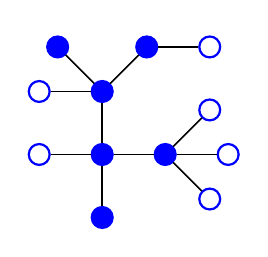
\begin{tikzpicture}[-, >=, auto, semithick, node distance=01cm]
\tikzstyle{every edge}=[segment length=1mm,segment angle=10, draw]

\tikzstyle{full node}=[circle, fill=blue,draw=blue,thick,text=black,scale=0.8]
\tikzstyle{light node}=[circle, fill=white,draw=blue,thick,text=black,scale=0.8]
\node[full node]    (1)                     {};
\node[full node]    (2)[above right of=1]         {};
\node[full node]    (3)[above left of=1]         {};
\node[full node]    (4)[below of=1]         {};
\node[full node]    (5)[right of=4]         {};
\node[full node]    (6)[below of=4]         {};
\node[light node]    (7)[left of=1]         {};
\node[light node]    (8)[right of=2]         {};
\node[light node]    (9)[left of=4]         {};
\node[light node]    (10)[above right of=5]         {};
\node[light node]    (11)[ right of=5]         {};
\node[light node]    (12)[ below right of=5]         {};
% \node[light node]    (4)[above of=2]         {};
\path

(1) edge node{} (2)
    edge node{} (3)
    edge node{} (7)
    ;
\path
(5) edge node{} (10)
    edge node{} (11)
    edge node{} (12)
    ;
    \path
(4) edge node{} (5)
    edge node{} (1)
    edge node{} (9)
    edge node{} (6)
    ;
    \path
(2) edge node{} (8)   
    ;
\end{tikzpicture}
\end{center}
\caption{Un réseau fait de noeuds lourds (bleu) et de noeuds légers (blanc)}
\label{fig:blockchain_network}
\end{figure}
Les noeuds légers se contentent d'émettre des informations (appelées transactions). Les noeuds lourds doivent vérifier la cohérence des transactions et s'accorder sur les informations à inscrire dans la blockchain. Les noeuds lourds appliquent un protocole de consensus pour se mettre d'accord. La preuve de travail ou \textit{Proof-of-Work} est le protocole utilisé dans le cadre de la blockchain des bitcoins, voir le whitepaper de \citet{Nakamoto2008}. Un bloc doit être ajouté toutes les dix minutes environ, les noeuds sont en compétition pour résoudre un problème cryptographique brutalement via une méthode essai-erreur (\textit{trial and error}). Le premier qui parvient à résoudre le problème ajoute le bloc et récupère une récompense d'un montant de BTC$6.25$ à l'heure de l'écriture.\footnote{\url{https://bitcoinblockhalf.com/}}. \\

Dans la blockchain des bitcoins, les informations enregistrées sont des échanges de bitcoin entre les participants. Un noeud peut facilement émettre deux transactions conflictuelles, c'est à dire qui transfèrent les mêmes unités à deux entités différentes. Il s'agit d'une attaque par double dépense. Le scénario standard est le suivant:
\begin{enumerate}
    \item Marie transfère à John BTC$10$
    \item La transaction de Marie à John est enregistrée dans la blockchain
    \item John doit atendre $\alpha\in\N$ confirmations, c'est à dire que $\alpha$ blocs soient ajoutés après celui dans lequel la transaction de Marie à John est inscrite
    \item Une fois que $\alpha$ confirmations ont été envoyées, John envoie le bien à Marie
    \item Pendant ce temps, Marie travaille sur sa propre version de la blockchain (dite privée) dans laquelle la transaction de Marie à John est remplacée par une transaction de Marie à elle même
    \item Au moment de la livraison du bien la blockchain dite principale est en avance de $z$ blocs 
    \item L'objectif de Marie est générer une chaine concurrente plus longue que la chaine principale. Si elle y parvient, elle la communiquera à l'ensemble du réseau pour créer une fourche (\textit{fork}). Le réseau optera alors pour la branche la plus longue.
    La branche de Marie va alors remplacer la branche principale permettant à Marie de récupérer ses unités qu'elle peut dépenser à nouveau. 
\end{enumerate}
Cette course entre les deux branches est résumée sur la \cref{fig:dp_illustration}.
\begin{figure}[ht!]
\begin{center}
\begin{tikzpicture}[-, >=stealth', auto, semithick, node distance=1cm]
% \tikzstyle{block} = [rectangle, draw, fill=blue!20,
%     text width=5em, text centered, rounded corners]
\tikzstyle{block}=[rectangle, fill=black,draw=black,thick,text=black,scale=1.5]
\tikzstyle{block}=[rectangle, fill=white,draw=black,thick,text=black,scale=1.5]
\tikzstyle{confirmed block}=[rectangle, fill=white,draw=blue,thick,text=black,scale=1.5]
\tikzstyle{bad block}=[rectangle, fill=white,draw=red,thick,text=black,scale=1.5]
\node[block]    (1)                     {\tiny $\text{M}\rightarrow \text{J}$};
\node[block]    (2)[right of=1]                     {};
\node[block]    (3)[right of=2]                     {};
\node[block]    (4)[right of=3]                     {};
\node[confirmed block]    (5)[right of=4]                     {};

\node[bad block]    (6)[below of=1]         {\tiny $\text{M}\rightarrow \text{M}$};
\node[block]    (7)[right of=6]         {};
\node[block]    (8)[right of=7]         {};
\path
(1) edge[ left]     node{}     (2)
(2) edge[ left]     node{}     (3)
(3) edge[ left]     node{}     (4)
(4) edge[ left]     node{}     (5)
(6) edge[ left]     node{}     (7)
(7) edge[ left]     node{}     (8);

\end{tikzpicture}
\end{center}
\caption{La course à la double dépense illustrée, ici nous avons $\alpha = 4$ et $z = 2$}
\label{fig:dp_illustration}
\end{figure}
Notre objectif est de calculer la probabilité que la branche de Marie devienne majoritaire. Soit $(Z_n)_{n\in\mathbb{N}}$ la différence de longueur entre la branche de Marie et la branche principale de la blockchain. On a $Z_0 = z\geq 0$ et la double dépense se produit à l'instant aléatoire
\begin{equation}\label{eq:dp_time}
\tau_0 = \inf\{n\geq0\text{ ; }Z_n = 0\}.
\end{equation}
Nous souhaitons étudié la distribution de $\tau_0$ et en particulier calculer la probabilité de double dépense définie par 
\begin{equation}\label{eq:dp_prob}
\phi(z) = \Prob(\tau_0 <\infty|Z_0 = z) := \Prob_z(\tau_0 <\infty)
\end{equation}
A chaque instant $k\in\N$ un bloc est ajouté, il appartient 
\begin{itemize}
    \item A la branche principale avec probabilité $p\in(0,1)$
    \item à la branche de Marie avec probabilité $1-p$
\end{itemize}
Soit $(\Omega,\F, \Prob)$ un espace probabilisé. On définit une suite $(\xi_n)_{n\geq0}$ \iid de variables aléatoires (\va) de loi 
$$
\mathbb{P}(\xi = 1) = p\text{, et }\mathbb{P}(\xi = -1) = 1-p.
$$
On en déduit que 
$$
Z_n = z +\sum_{k=1}^n\xi_k.
$$
Le processus $Z_n$ est un processus à temps discret et à valeur dans $\Z$. Une visualisation du problème de premier passage est donné sur la \cref{fig:double_spending_time}.
\begin{figure}[ht!]
\begin{center}
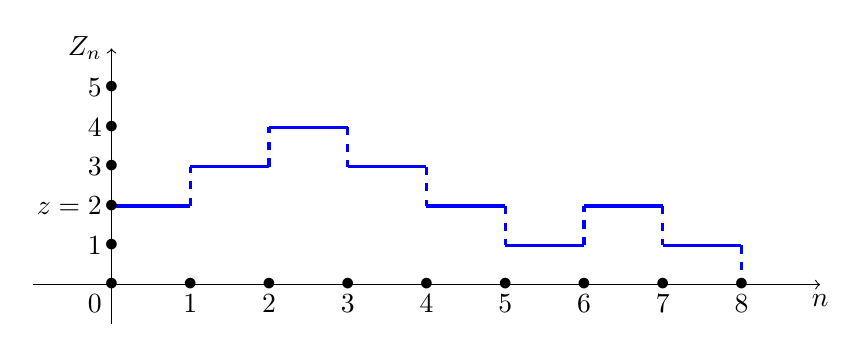
\begin{tikzpicture}
  %Origin and axis
  \coordinate (O) at (0,0);
  \draw[->] (-1,0) -- (9,0) coordinate[label = {below:$n$}] (xmax);
  \draw[->] (0,-0.5) -- (0,3) coordinate[label = {left:$Z_n$}] (ymax);
  %Lower linear boundary

 
  %Stochastic process trajectory
  
  \draw (0,0) node[blue,left] {} node{};
  \draw[very thick,blue,-] (0,1) -- (1,1) node[pos=0.5, above] {} ;
  \draw[very thick,dashed,blue] (1,1) -- (1,1.5) node[pos=0.5, right] {};
  \draw[very thick,blue,-] (1,1.5) -- (2,1.5) node[pos=0.5, above] {};
  \draw[very thick,dashed,blue] (2,1.5) -- (2,2) node[pos=0.5, right] {};
  \draw[very thick,blue,-] (2,2) -- (3,2) node[pos=0.5, above] {};
  \draw[very thick,dashed,blue] (3,2) -- (3,1.5) node[pos=0.5, right] {};
  \draw[very thick,blue,-] (3,1.5) -- (4,1.5)node[pos=0.5, above] {};
  \draw[very thick,dashed,blue] (4,1.5) -- (4,1) node[pos=0.5, right] {};  
  \draw[very thick,blue,-] (4,1) -- (5,1) node[pos=0.5, above] {};
  \draw[very thick,dashed,blue] (5,1) -- (5,0.5) node[pos=0.5, right] {};  
  \draw[very thick,blue,-] (5,0.5) -- (6,0.5) node[pos=0.5, above] {};
  \draw[very thick,dashed,blue,-] (6,0.5) -- (6,1) node[pos=0.5, above] {};
   \draw[very thick,blue,-] (6,1) -- (7,1) node[pos=0.5, above] {};
    \draw[very thick,dashed,blue,-] (7,1) -- (7,0.5) node[pos=0.5, above] {};
     \draw[very thick,blue,-] (7,0.5) -- (8,0.5) node[pos=0.5, above] {};
     \draw[very thick,dashed,blue,-] (8,0.5) -- (8,0) node[pos=0.5, above] {};
  %Jump Times
  \draw (1,0) node[black,below] {$1$} node{ \color{black}$\bullet$};
  \draw (2,0) node[black,below] {$2$} node{ \color{black}$\bullet$};
  \draw (3,0) node[black,below] {$3$} node{ \color{black}$\bullet$};
  \draw (4,0) node[black,below] {$4$} node{ \color{black}$\bullet$};
  \draw (5,0) node[black,below] {$5$} node{ \color{black}$\bullet$};
  \draw (6,0) node[black,below] {$6$} node{ \color{black}$\bullet$};
  \draw (7,0) node[black,below] {$7$} node{ \color{black}$\bullet$};
  \draw (8,0) node[black,below] {$8$} node{ \color{black}$\bullet$};
  %Level of the counting process
   \draw (0,0) node[black,below left] {$0$} node{ \color{black}$\bullet$};
   \draw (0,0.5) node[black,left] {$1$} node{ \color{black}$\bullet$};
   \draw (0,1) node[black,left] {$z=2$} node{ \color{black}$\bullet$};
   \draw (0,1.5) node[black,left] {$3$} node{ \color{black}$\bullet$};
   \draw (0,2) node[black,left] {$4$} node{ \color{black}$\bullet$};
   \draw (0,2.5) node[black,left] {$5$} node{ \color{black}$\bullet$};

  % %Aggregated Capital gains
%  \draw (0,1.5) node[blue,below right] {$\mu_1$} node{ \color{blue}$-$};
%  \draw (0,2.25) node[blue,left] {$\mu_2$} node{ \color{blue}$-$};
%  \draw (0,3.75) node[blue,left] {$\mu_3$} node{ \color{blue}$-$};
  %Ruin time = First-crossing time time
%  \draw (5,0) node[black,above right] {${\tau_0}_u$} node{ \color{black}$\times$};
%  \draw[dotted,black] (0,3.28) -- (5,3.28);
%  \draw[dotted,black] (5,0) -- (5,3.28);
\end{tikzpicture}
\end{center}
\caption{Illustration du problème de premier passage sous-jacent à la double dépense.}
\label{fig:double_spending_time}
\end{figure}
L'application du \cref{theo_ruin_proba} avec $a\rightarrow \infty$ permet de résoudre le problème avec 
$$
\phi(z) = \left(\frac qp\right)^z.
$$

% \section{Annexes: Récurrence de la marche aléatoire sur $\mathbb{Z}$}\label{app:recurrence}

\section{Annexes: Convergence des Martingales}\label{app:convergence_martingale}
Cette section présente des résultats sur l'existence d'une loi limite pour les processus martingales. Soit $X=(X_n)_{n\geq 0}$ un processus défini sur un espace $(\Omega, \mathcal{F},\mathbb{P})$ adapté à la filtration $\mathcal{F}_n$ tel que $X_n$ est intégrable pour tout $n\geq 0$.
\begin{theo}\label{theo:convergence_ps_martingale}[De convergence des martingales]
Si $(X_n)_{n\geq0}$ est une S-martingale bornée dans $L^1$, c'est à dire telle que 
$$
\underset{n\in\mathbb{N}}{\sup}\E[(X_n)_+]<\infty,
$$ 
alors $X_n$ converge presque sûrement et dans $L^1$ vers une \va intégrable $X_\infty$.

\end{theo}
\begin{proof}
La démonstration du résultat nécessite de montrer un lemme pour lequel nous avons besoin d'introduire les objets suivants. Soit $a<b$ deux réels, on note 
\begin{itemize}
    \item $S_0 = T_0 = 0$,
    \item $S_1 = \inf\{n\geq 0\text{ : }X_n\leq a\}$ et $T_1 = \inf\{n> S_1\text{ : }X_n\geq b\}$,
    \item $S_{m+1} = \inf\{n> T_m\text{ : }X_n\leq a\}$ et $T_{m+1} = \inf\{n> S_m\text{ : }X_n\geq b\}$,
\end{itemize}
Pour tout $N\in \mathbb{N}$, on pose $M  = \sup\{m\geq 0, T_m \geq N\}$, noté $M_{N}(a,b)$ qui correspond au nombre de traversées montantes de l'intervalle $(a,b)$ par le processus $X$ jusqu'au temps $N$, en effet, on a 
$$
X_{S_{1}}\leq a,\,X_{T_{1}}\geq b,\ldots, X_{S_{M}}\leq a,  X_{T_{M}}\geq b.
$$

\begin{lemma}
Si $X$ est une sur-martingale alors 
$$
(b-a)\E\left[M_N(a,b)\right]\leq \E[(X_N-a)_
{-}],
$$
où $(x)_{-} = -\min(0,x)$ est la partie négative de $x$.

\end{lemma}
\begin{proof}
TODO
\end{proof}
Montrons le théorème dans le cas d'une sur-martingale . Le cas d'une sous-martingale s'en déduit car si $X$ est unue sous-martingale, bornée dans $L^1$ alors $Y  = -X$ est une sur-martingale bornée dans $L^1$ et le résultat s'applique. Pour une trajectoire $n\mapsto X_n(\omega)$ jusqu'au temps, le nombre de traversées montante $M_N(a,b)$ est une suite croissante en $N$, on note 
$$
M(a,b) = \underset{N\geq 0}{\sup} M_N(a,b).
$$ 
On remarque que 
$$
(b-a)\E[M_N(a,b)]\leq \E[(X_n-a)_{-}]\leq\E(|X_N|) + |a|\leq  \underset{N\geq 0}{\sup}\E(|X_N|) + |a|<\infty
$$
Cela implique qie $M(a,b)$ est fini presque surement. Si $X$ ne converge pas dans $\overline{\mathbb{R}} = \mathbb{R}\cup \{-\infty, +\infty\}$ lorsque $n\rightarrow\infty$ pour une trajectoire $\omega$, alors on a 
$$
\underset{n\rightarrow \infty}{\liminf}\, X_n(\omega) < \underset{n\rightarrow \infty}{\limsup}\, X_n(\omega). 
$$
Il existe alors deux rationnels $a<b$ tels que 
$$
\underset{n\rightarrow \infty}{\liminf}\, X_n(\omega) < a < b \underset{n\rightarrow \infty}{\limsup}\, X_n(\omega). 
$$
Dans ce cas $M(a,b) = \infty$, cela signifie que $\omega$ appartient à un ensemble de probabilité nulle. Par contraposée, le processus $X$ converge sauf sur des ensemble de mesure nulle et donc presque surement. De plus, on a 
$$
\E(|X_\infty|) = \E(\underset{n\rightarrow\infty}{\lim} |X_n|) = \E(\underset{n\rightarrow\infty}{\liminf} \,|X_n|)\underset{\text{Lemme de Fatou}}{\leq} \underset{n\rightarrow\infty}{\liminf}\,\E( |X_n|)\leq \underset{n\geq 0}{\sup}\,\E(|X_n|)< \infty.
$$

\end{proof}
On déduit du théorème précédent le corollaire suivant:
\begin{coro}
Soit $X$ une sur-martingale positive alors 
$$
X_\infty := \underset{n\rightarrow\infty}{\lim} X_n\text{ existe presque surement,}
$$
et vérifie $X_n \geq  \E(X_\infty|\F_n)$.
\end{coro}
\begin{proof}
Une sur-martingale positive est bornée dans $L^1$ donc le \cref{theo:convergence_ps_martingale} s'applique.
\end{proof}
Dans la suite nous avons besoin de la notion d'uniforme intégrabilité (UI). 
\begin{definition}
Le processus $X$ est uniformément intégrable (UI) si 
$$
\underset{M\rightarrow\infty}{\lim}\,\underset{n\geq 0}{\sup}\,\E(|X_n|\mathbb{I}_{|X_n|>M}) = 0
$$
Cela équivaut à 
$$
\forall \epsilon >0, \exists M >0,\forall n\geq 0,  \E(|X_n|\mathbb{I}_{|X_n|>M}) <\epsilon
$$
\end{definition}
\begin{ex}
Un processus $X$ dominé par une \va intégrable $Y$ est UI. En effet, pour tout $n\geq 0$
$$
\E(|X_n|\mathbb{I}_{[|X_n|>M})\leq \E(|Y|\mathbb{I}_{[|X_n|>M})\leq \E(|Y|\mathbb{I}_{[|Y|>M})
$$
On note que $\E(|Y|) = \E(|Y|\mathbb{I}_{|Y|\leq M} + \mathbb{I}_{|Y|>M})$ et $\underset{M\rightarrow \infty}{\lim}\, \E(|Y|\mathbb{I}_{[|Y|\leq M}) = \E(|Y|)$ cela implique que  
$$
 \underset{M\rightarrow \infty}{\lim}\E(|Y|\mathbb{I}_{[|Y|>M}) = 0.
$$
En particulier, le processus 
$$
X_n = \E(Y|\mathcal{F}_n),\text{ }n\geq 0,
$$
est une martingale UI.
\end{ex}
Une notion proche de l'uniforme intégrabilité est l'équi-intégrabilité
\begin{definition}
Le processus $X$ est equi-intégrable (EI) si 
$$
\forall \epsilon >0, \exists \eta >0, \forall A\in\mathcal{F}, \forall n\geq 0,\Prob(A)<\eta\Rightarrow \E(|X|\mathbb{I}_A) <\epsilon
$$
\end{definition}
La convergence des martingales est liée au fait que le processus soit bornée dans $L^1$, le résultat fait le lien entre uniforme intégrabilité et le fait que $X$ soit borné dans $L^1$. 
\begin{prop}
Soit $X$ un processus intégrable, les assertions suivantes sont intégrables 
\begin{itemize}
    \item[(i)] $X$ est UI
    \item[(ii)] $X$ est borné dans $L^1$ et $X$ est EI.
\end{itemize}
\end{prop}
\begin{proof}
TODO
\end{proof}
La notion d'uniforme intégrabilité permet de faire le pont entre convergence dans $L^1$ et convergence en probabilité. 
\begin{theo}
Soit $X$ un processus et $X_\infty$ une \va intégrable, les assertions suivantes sont équivalentes
\begin{itemize}
    \item[(i)] $X$ est UI et $X_n\overset{\Prob}{\rightarrow} X_{\infty}$. 
    \item[(ii)] $X$ est intégrable et $X_n\overset{L^1}{\rightarrow} X_{\infty}$. 
\end{itemize}
\end{theo}
\begin{proof}
TODO
\end{proof}
Avant de poursuivre, on introduit la notion de S-martingale fermée.
\begin{definition}
Une S-martingale $X$ est fermée à droite par une \va intégrable $Z$ si 
$$
\E(Z|\F_n)= X_n (\text{resp }\geq X_n\text{ ou }\leq X_n) 
$$
dans le cas d'une martingale (resp. d'une sous ou sur - martingale)
\end{definition}
On peut connecter la notion de martingale fermée et UI via le résultat suivant 
\begin{prop}
Soit $Z$ une \va intégrable alors la martingale définie par 
$$
X_n  = \E(Z|\F_n)
$$
est UI. 
\end{prop}
\begin{proof}
On a $X_n \leq Z_n  = \E(Z|\F_n)$, on a pour tout $n\geq 0$, 
$$
\E(X_n\mathbb{I}_{|X_n|>M})\leq \E(Z_n\mathbb{I}_{|Z_n|>M}) = \E(|Y|\mathbb{I}_{|Z_n|>M})
$$
Il faut démontrer que 
$$
\underset{M\rightarrow \infty}{\lim}\underset{n\geq 0}{\sup}\,\E(|Y|\mathbb{I}_{|Z_n|<M}).
$$
On a, pour $N, M>0$ 
\begin{eqnarray*}
\E(|Y|\mathbb{I}_{|Z_n|>M})&=& \E(|Y|\mathbb{I}_{|Z_n|>M, |Y|\leq N}) + \E(|Y|\mathbb{I}_{|Z_n|>M, |Y|> N})\\
&\leq& N \Prob(|Z_n|>M) + \E(|Y|\mathbb{I}_{|Y|> N})\\
&\underset{\text{Markov}}{\leq}& N\frac{\E(|Z_n|)}{M} + \E(|Y|\mathbb{I}_{|Y|> N})\\
&\underset{\text{Jensen}}{\leq}& N\frac{\E(|Y|)}{M} + \E(|Y|\mathbb{I}_{|Y|> N})\\
\end{eqnarray*}
pour tout $\epsilon >0$, il existe $N$ tel que $\E(|Y|\mathbb{I}_{|Y|> N})<\epsilon / 2$ (comme $Y$ est intégrable, c'est possible). On choisit alors $M =\frac{\E(2|Y|)N}{\epsilon}$, il vient 
$$
\underset{n\geq 0}{\sup}\,\E(|Y|\mathbb{I}_{|Z_n|<M})\leq \epsilon.
$$
\end{proof}
On peut énoncer le théorème de convergence suivant 
\begin{theo}
Soit $X$ une S-martingalme alors 
$$
X_n\overset{ L^1}{\longrightarrow}X_\infty\Leftrightarrow
 X\text{ est UI}$$
 Dans ce cas, $X$ converge presque sûrement vers $X_\infty$ et est fermée à droite par $X_\infty$
\end{theo}
\begin{proof}
TODO
\end{proof}
\begin{coro}
Soit $X$ une martingale, Les assertions suivnates sont équivalentes
\begin{itemize}
    \item[(i)] $X$ est UI
    \item[(ii)] $X_n\overset{ L^1}{\longrightarrow}X_\infty$
    \item[(iii)] $X$ est fermée à droite : $\exists Z\in L^1, \forall n\geq 0, \E(Z|\F_n) = X_n$
\end{itemize}
\end{coro}
\begin{proof}
TODO
\end{proof}
On peut aussi énoncer uun théorème d'arrêt avec des temps d'arrêt quelconques (pas nécessairement bornés)
\begin{theo}
Supposons que $X$ est une S-martingale UI alors pour deux temps d'arrêt (quelconques) tels que $\sigma\leq \tau$, on a 
$$
\E(X_\tau|\F_\sigma)= X_\sigma (\text{resp }\geq X_\sigma\text{ ou }\leq X_\sigma) 
$$
dans le cas d'une martingale (resp. d'une sous ou sur - martingale). En zparticulier, on a 
$$
\E(X_\infty|\F_\sigma) = X_\sigma.
$$
\end{theo}
\begin{proof}
TODO
\end{proof}

% \bibliography{includes/calcul_sto_chap_I}
% \bibliographystyle{plainnat}
% \section{Annexes: Un problème de contrôle optimal}
% La richesse d'une entreprise est modélisée par la marche aléatoire suivante
% $$
% X_{n+1} = X_n +\xi_{n+1}, \text{ }n\geq 0
% $$
% avec $X_0 = x$ et $(\xi_{n})_{n\geq1}$ une suite de \va \iid. On va supposer que $c\in\mathbb{N}$ et que les $\xi_i$ sint de \va discrète à valeurs dans $\mathbb{Z}$ telles que 
% $$
% \Prob(\xi_1 = i) = p_i\text{, }i\in\mathbb{Z},
% $$
% de sorte que $X_n\in \mathbb{Z}$. C'est un modèle doublement discret (en temps et en espace). Une partie de la richesse de l'entreprise doit être reversé aux actionnaire à cahque pas de temps sous la forme de dividende vu comme une suite de \va notée $(D_n)_{n\geq 0}$. Cela modifie la richesse de l'enstreprise qui devient 
% \begin{equation}\label{eq:controlled_process}
% \tilde{X}_{n+1} = \tilde{X}_n - D_n +\xi_{n+1}, \text{ }n\geq 0.
% \end{equation}
% Le montant de dividende est à la discrétion des dirigeants de l'entreprise et se réduit à une fonction $w$ telle que 
% $$
% D_n = w(\tilde{X}_n)<\tilde{X}_n.
% $$
% Le processus $(\tilde{X}_n)_{n\geq0}$ est le processus de richesse dit contrôlé, où $D_n$ est le contrôle. Soit 
% $$
% \tau_0 = \inf\{n\geq 0\text{ ; }X_n =0\},
% $$
% le temps de ruine, premier instant pour lequel la richesse modifiée pass en dessous de $0$. Soit $\delta>0$ le facteur d'actualisation et 
% $$
% V(x,w) =\E\left(\sum_{n =0}^{\tau- 1 }\delta^n D_n\right),
% $$
% l'espérance du cumul du montant actualisé des dividendes jusqu'à la cessation d'activité (ici la banqueroute). L'objectif des dirigeants est de définir une stratégie $w$ qui maximise $V(x,w)$, c'eest à dire permettant d'atteindre la cible 
% $$
% V(x) = \underset{w}{\sup} V(x,w).
% $$
% \begin{definition}\label{def:undominated_strategy}
% Une stratégie $w^\ast$ domine une startégie $w$ si 
% \begin{enumerate}
%     \item $V(x,w^\ast)\geq V(x,w)$ pour tout $x\geq 0$
%     \item $V(x,w^\ast)> V(x,w)$ pour certain $x\geq 0$
% \end{enumerate}
% Une stratégie "dominante" n'est dominée par aucune autre stratégie. 
% \end{definition}

% \subsection{ Exemple de stratégie}
% Une stratégie classique est du type \textit{band}.
% \begin{definition}
% Une \textit{band strategy} est la donnée de $2k+1$ entiers $a_0 <b_1<a_2<\ldots <b_n< a_n$ de sorte que le montant de dividendes versé aux actionnaires est défini par 
% $$
% D_n = w(\tilde{X}_n) = \begin{cases}
% 0,&\text{ si }\tilde{X}_n \geq a_0\text{ et }b_l\leq \tilde{X}_n\leq a_l\text{ pour }l = 1,\ldots, k.\\
% \tilde{X}_n - a_{l-1},&\text{ si }a_{l-1}\leq \tilde{X}_{n}\leq b_l\text{ pour }l = 1,\ldots, k,\\
% \tilde{X}_n - a_{k}, &\text{ si }\tilde{X}_{n} > a_{k}.
% \end{cases}
% $$
% \end{definition}
% La \textit{band strategy} est illustrée sur le schéma \cref{fig:band_strategy} avecc une trajectoire de $(\tilde{X}_n)_{n\geq 0}$.
% \begin{figure}[!ht]
% \begin{center}
% \begin{tikzpicture}
%     \begin{axis}[
%         axis lines = left,
%         xlabel = Time,
%         ylabel = {Capital},
%         ymin=0, ymax=140,
%         xmin=0, xmax=10,
%         ytick={30,60,90,120},
%         yticklabels={$a_0$, $b_1$, $a_1$, $b_2$},
%         xtick={0,1,...,9},
%         clip=false,
%         ]

%         % Upper and lower band lines
%         \addplot[domain=0:10, color=red, dashed] {120};
%         \addplot[domain=0:10, color=blue, dashed] {90};
%         \addplot[domain=0:10, color=green, dashed] {60};
%         \addplot[domain=0:10, color=orange, dashed] {30};

%         % Capital over time as a random walk
%         \addplot[mark=*,mark options={fill=black}] coordinates {
%             (0,50) (0,30) (1,65) (2,80) (3,70) (4,100) (4,90) (5,75) (6,80) (7,50) (7,30) (8,130) (9,110) (9,90) (10,85)
%         };

%         % Dividend payout points
%         % \draw[dashed] (axis cs:7,85) -- (axis cs:7,60);
%         % \draw[dashed] (axis cs:8,90) -- (axis cs:8,60);

%         % \node at (axis cs:7,25) [anchor=north] {Dividend Payout};
%         % \node at (axis cs:8,25) [anchor=north] {Dividend Payout};
%     \end{axis}
% \end{tikzpicture}
% \end{center}
% \caption{Trajectoire du processsus contrôlé $(\tilde{X}_n)_{n\geq 0}$.}
% \label{fig:band_strategy}
% \end{figure}

% \noindent L'existence d'une \textit{band strategy} optimale dans le cadre de notre modèle a été prouvé par exemple dans \citet[Theorem 1]{Gerber1972}. Il n'est cependant pas évident de trouver les bornes définissant les bandes explicitement. C'est plus facile dans le cas où $k=0$ qui correspond à une stratégie dite barrière. Lorsque la richesse excède le seuil $a:=a_0$, le surplus est reversé aux actionnaires. L'existence d'une stratégie barrière a été démontré dans le travail de \citet{Miyasawa1961} lorsque 
% $$
% p_i = 0\text{ pour } i \leq -2.
% $$
% Dans \citet{Gerber1972}, il est démontré l'existence qu'une stratégie barrière de niveau $a$ est localement optimale c'est à dire optimale pour certain niveau de capital initial $x =0,\ldots, a$, lorsque 
% $$
% p_i = 0\text{ pour } i \geq 2.
% $$
% On va se contenter d'établir l'optimalité de la stratégie barrière dans le cas d'une marche aléatoire simple dans la section \cref{subsec:optimality_band_strategy}
% La détermination explicite du seuil de la barrière et du montant espéré des dividendes est effectuée dans la section \cref{subsec:dividen_RW}.
% \subsection{Optimalité de la stratégie barrière dans le cas de la marche aléatoire simple}\label{subsec:optimality_band_strategy}
% On suppose que 
% $$
% \Prob(\xi_1 = 1) = p,\text{ }\Prob(\xi_1 = 1) = q = 1-p.
% $$
% La stratégie dominante $w^{\ast}$ doit vérifier l'équation suivante 
% \begin{equation}\label{eq:bellman_equation}
% V(x,w^\ast) = \max\left[\delta (pV(x+1,w^\ast) + qV(x-1,w^\ast)), \underset{1\leq y\leq x}{\max} y + V(x-y,w^\ast)\right],
% \end{equation}
% qui indique que l'entreprise au vu de son niveau de surplus peut entrer dans le nouvelle exercice en ne versant pas de dividendes ou en versement directement un montant 
% $$
% w^{\ast}(x) = y.
% $$
% L'équation fonctionnelle \eqref{eq:bellman_equation} est l'équation vérifié par $V$ est appelée équation de Bellman. Il s'agit d'une application du principe de la programation dynamique qui exprime que la solution optimale est déterminer par une stratégie permettant de passer d'une période à une autre. Il est possible que les termes $\delta (pV(x+1,w^\ast) + qV(x-1,w^\ast))$ et  $\underset{1\leq y\leq x}{\max} y + V(x-y,w^\ast)$ soient égaux, nous adoptons la convention suivante 
% \begin{equation}\label{eq:strategie_speciale}
% w^\ast(x) = 0 \Leftrightarrow \delta (pV(x+1,w^\ast) + qV(x-1,w^\ast)) >  \underset{1\leq y\leq x}{\max} y + V(x-y,w^\ast)
% \end{equation}
% qui stipule qu'en cas d'égalité, on préfère payer des dividendes immédiatement. On peut ré-écrire \eqref{eq:bellman_equation} comme 
% \begin{equation}\label{eq:eq:bellman_equation2}
% V(x,w^\ast) =  \underset{0\leq y\leq x}{\max} y +  h(x-y, \omega^\ast), 
% \end{equation}
% où
% $$
% h(x, \omega^\ast) = \delta\left[ pV(x+1,w^\ast) + qV(x-1,w^\ast)\right].
% $$
% \begin{prop}\label{prop:properties_optimal_strategy}
% Soit $w^\ast$ une stratégie dominante.
% \begin{enumerate}
%     \item Il existe $x\in \mathbb{N}$ tel que $w^\ast(x) >0$
%     \item S'il existe $x,a$ et $b$ des entiers tels que $a<b$ et 
%     $$
%     w^\ast(x)=\begin{cases}
%     0,&\text{ pour }x \leq a, \\
%     >0,&\text{ pour }a<x <b,
%     \end{cases}
%     $$
%     alors 
%     $$
%     w^\ast(x)=\begin{cases}
%             0,&\text{ pour }x \leq a, \\
%             x-a,&\text{ pour }a<x\ <b,\\
%             \end{cases}
%             $$
% \end{enumerate}
% \end{prop}
% \begin{proof}
% \begin{enumerate}
%     \item Supposons que $w^\ast(x) = 0$ pour tout $x$ alors $V(x,w^\ast) = 0$. Or la stratégie $w'$ qui consiste à verser l'intégralité du capital restant en dividende est tel que 
%     $$
%     V(x,w') = x > V(x,w^\ast)\text{, pour }x\geq 1.
%     $$
%     ce qui contredit la domination bde $w^\ast$.
%     \item Par hypothèse $w^\ast(a) = 0$, on en déduit que 
% $$
% V(a,w^\ast) = \underset{y = 0,\ldots, a}{\max} y + h(a-y,w^\ast) = h(a,w^\ast).
% $$
% On considère 
% \begin{eqnarray*}
% V(a+1,w^\ast) &=& \underset{y = 0,\ldots, a+1}{\max} y + h(a+1-y,w^\ast))\\
% &=&\max(h(a+1,w^\ast), \underset{y = 1,\ldots, a+1}{\max} y + h(a+1-y,w^\ast))\\
% &=&\max(h(a+1,w^\ast), \underset{y = 0,\ldots, a}{\max} y +1 + h(a-y,w^\ast))\\
% &=&\max(h(a+1,w^\ast), 1+h(a,w^\ast))
% \end{eqnarray*}

% En itérant jusqu'à k tel que $a+k = b-1$ il vient 
% $$
% w^\ast(a+l) =l,\text{ pour }l = 1,\ldots, k.
% $$
% On a pour finir 

% \begin{eqnarray*}
% V(b,w^\ast) &=& \underset{y = 0,\ldots, a+1}{\max} y + h(b-y,w^\ast))\\
% &=&\max(h(b,w^\ast), \underset{y = 1,\ldots, a+1}{\max} y + h(a+1-y,w^\ast))\\
% &=&\max(h(a+1,w^\ast), \underset{y = 0,\ldots, a}{\max} y +1 + h(a-y,w^\ast))\\
% &=&\max(h(a+1,w^\ast), 1+h(a,w^\ast)).
% \end{eqnarray*}
% \end{enumerate}

% \end{proof}
%  La proposition indique l'existence d'un plus petit entier $a$ qui joue le rôle de barrière réfléchissante. La question est de savoir s'il existe $b >a$ tel que $w^\ast(b) = 0$ auquel cas on aurait aussi l'existence de $a_1>b$ tel que $w(a_1+1)>0$ par l'item $1$ et de plus $w(a_1+1) = 1$ par l'item $2$. On peut postuler une stratégie dominante telle que 
%  $$
% w^\ast(x)=\begin{cases}
%             0,&\text{ pour }x \leq a, \\
%             x-a,&\text{ pour }a<x\ <b,\\
%             0,& \text{ pour }b\leq x\leq a_1\\
%             1,\text{ pour }x = a_1+1
%             \end{cases}
%  $$
%  Il s'agit d'un embryon de stratégie de type bande. Pour que cette stratégie soit de type barrière il faut montrer que $b = \infty$. C'est l'objet du réusltat suivant. 
%  \begin{theo}
%  Dans le cas où la richesse est gouvernée par une marche aléatoire simple, on a $b = \infty$

%  \end{theo}
%  \begin{proof}
%  Supposons qu'il existe $b <\infty$ alors il existe également $a_1<\infty$ tel que $a_1>b$. On va montrer que l'on peut définir une stratégie $w'$ qu domine $w^\ast$. Notons $\tilde{X}^\ast_n$ et $\tilde{X}'_n$ les processus contrôlés en appliquant les stratégies $w^\ast$ et $w'$ respectivement. On note 
%  $$
%  \tau' = \inf\{n\geq 0\text{ ; }\tilde{X}'_n  = a_1\},
%  $$
%  et
% $$
%  \tau^\ast = \inf\{n\geq 0\text{ ; }\tilde{X}^\ast_n  = b\}.
%  $$

%  Soit 
%  $$
% w'(\tilde{X}'_n)=\begin{cases}
%             0,&\text{ pour }\tilde{X}'_n \leq a,\text{ ou }n = \tau' ,\\
%             \tilde{X}'_n-a,&\text{ pour }a<\tilde{X}'_n\ <b- 1,\text{  et } n <\tau', \\
%             \tilde{X}'_n-a,&\text{ pour }a\leq\tilde{X}'_n\leq b,\text{  et } n \geq \tau', \\
%             0,&\text{ pour }b-1<\tilde{X}'_n\ <a_1,\text{  et } n <\tau', \\
%             0,& \text{ pour }b\leq \tilde{X}'_n\leq a_1,\text{  et } n \geq \tau',\\
%             w^\ast (\tilde{X}'_n),&\text{ pour }\tilde{X}'_n = a_1+1.
%             \end{cases}
% $$

%  \end{proof}
%  Supposons que $X_0' = x$ et  $X_0^\ast = x+1$ avec $b\leq x <x+1\leq a_1$. On considère le scénario dans chacune des deux situations, c'est à dire des valeurs identiques pour les éléments de la suite $(\xi_n)_{n\geq 0}$. On étudie deux cas séparément. 

% \begin{enumerate}
%     \item Supposons que $X_n'$ atteigne $a_1$ (c'est l'instant $\tau'$) avant que $X_n^\ast$ n'atteigne le niveau $b-1$. On a $X{_\tau'}^\ast = X{_\tau'}^\ast$ et même $X_n' = X_n^\ast$ pour $n\geq \tau'$ puisque $w^\ast$ et $w'$ coincide. On observe que 
%     $$
%     V(x+1,w^\ast) - V(x,w') = \delta^{\tau'} \leq 1
%     $$
%     \item Supposons que $X_n'$ n'atteigne pas $a_1$ avant que $X_n^\ast$ n'atteigne le niveau $b-1$ (instant $\tau^\ast$). On a $X_{\tau^\ast} = X_{\tau^\ast}$ et même $X_n' = X_n^\ast$ pour $n\geq \tau^\ast$ puisque $w^\ast$ et $w'$ coincide. On observe que 
%     $$
%     V(x+1,w^\ast) - V(x,w') = \delta^{\tau^\ast} \leq 1
%     $$
% \end{enumerate}
% Dans les deux cas $w'$ domine $w^\ast$, en effet 
% $$
% V(x+1,w') - V(x,w') \geq 1
% $$
% et donc $V(x+1,w') \geq V(x+1,w^\ast)$. Cela contredit la domination de $w^\ast$. On a bien $b = \infty$.
% \begin{remark}
% La preuve est assez fastidieuse. Dans la pratique, une stratégie $w^\ast$ est optimale lorsque les deux condition suivantes sont vérifiées
% \begin{itemize}
%     \item[(i)] $V(x+1,w^\ast)\geq V(x,w^\ast) + 1$
%     \item[(ii)] $V(x,w^\ast)\geq h(x,w^\ast)$
% \end{itemize}
% Voir le raisonnement dans la preuve de 2. de \cref{prop:properties_optimal_strategy}. On peut alors déterminer la stratégie optimale en postulant cette stratégie puis en vérifiant que (i) et (ii) sont satisfaite. Il faut pour cela avoir une idée de la stratégie optimale, qui est souvent du type barrière ou bande pour les processus du type marche aléatoire ou processus de Lévy qui sont l'équivalent des marche aléatoire en temps continu (étudié dans le \cref{chap:processus_levy})
% \end{remark}
% \subsection{Détermination de la barrière optimale et du montant espéré de dividende pour la marche aléatoire sur $\mathbb{Z}$}\label{subsec:dividen_RW}
% Dans le cas de la marche aléatoire simple la stratégie optimale est une stratégie barrière de niveau $a$ pour laquel la fonction objectif vérifie
% $$
% V(x;a) = \delta\left[pV(x+1;a) + qpV(x-1;a)\right],\text{ pour }1\leq x\leq a.
% $$ 
% Il s'agit d'une équation récurrente linéaire d'ordre deux avec les conditions limites suivantes
% $$
% V(0;a) =0\text{ et }V(a+1; a) = 1 + V(a; a).
% $$
% Les solutions sont données par 
% $$
% V(x;a) = A_1 r_1^x + A_2 r_2^x,
% $$
% où $A_1$ et $A_2$ sont des constantes et $r_1$ et $r_2$ sont les racines du polynôme caractéristique
% $$
% \delta p r^2 - r + \delta q = 0.
% $$
% On en déduit que 
% $$
% r_1 = \frac{1 + \sqrt{\Delta}}{2\delta p }\text{, et }r_2 = \frac{1 - \sqrt{\Delta}}{2\delta p },
% $$
% avec $\Delta = 1 - 4 \delta^2p(1-p)$. Via les conditions limites, on obtient
% $$
% A_1 = -A_2\text{ et }A_1 = \frac{1}{(r_1^{a+1} -r_2^{a+1} ) - (r_1^{a} -r_2^{a} )}
% $$
% Il est intéressant d'observer que 
% $$
% V(x;a) = g(a)f(x),
% $$
% où
% $$
% g(a) = \frac{1}{(r_1^{a+1} -r_2^{a+1} ) - (r_1^{a} -r_2^{a} )}
% $$
% La valeur optimal du seuil coincide avec le maximum de la fonction $g$ et ne dépend pas de la réserve initiale $x$.
% \begin{remark}
% Une manière économique et probabiliste d'obtenir le résultat est de considérer la valeur actuelle probable d'un paiement de montant $1$ à l'instant 
% $$
% \tau_{a+1} = \inf\{n\geq 0\text{ }X_n = a\},
% $$
% sachant que $X_n = x\leq a$ et que la ruine ne s'est pas produite. On note
% $$
% C(x, a+1) = \E_x(\delta^{\tau_{a+1}}\mathbb{I}_{\tau_{a+1}<\tau_0}).
% $$
% La richesse de l'entreprise est une chaine de Markov homogène. de plus, comme $X_0 = 1$, $\tau_x < \tau_{a+1}$ pour $x\leq a+1$, alors on peut écrire
% \begin{eqnarray}\label{eq:factorization_formula}
% C(1, a+1) &=& \E_1(\delta^{\tau_{a+1}}\mathbb{I}_{\tau_{a+1}<\tau_0})\nonumber\\
% & = &\E_1\left[\E(\delta^{\tau_{a+1} - \tau_x + \tau_x}\mathbb{I}_{\tau_{a+1}<\tau_0}\mathbb{I}_{\tau_{x}<\tau_0}\rvert \mathcal{F}_{\tau_x})\right]\nonumber\\
% &=&\E_1\left[\delta^{\tau_x}\mathbb{I}_{\tau_{x}<\tau_0}\E(\delta^{\tau_{a+1} - \tau_x }\mathbb{I}_{\tau_{a+1}<\tau_0}\rvert \mathcal{F}_{\tau_x})\right]\nonumber\\
% &=&\E_1\left[\delta^{\tau_x}\mathbb{I}_{\tau_{x}<\tau_0}\right]\E_x[\delta^{\tau_{a+1}}\mathbb{I}_{\tau_{a+1}<\tau_0}]\nonumber\\
% &=&C(1, x)C(x, a+1).
% \end{eqnarray}
% On note 
% $$
% f(x) = \frac{1}{C(1,x)}\text{, } x\leq a,
% $$
% que l'on appelle la fonction d'échelle (en théorie de la fluctuation). Dans le cadre d'une stratégie barrière de niveau $a$ la fonction objectif vérifie
% $$
% V(x; a) = x-a+V(a+1; a)\text{, pour }x\geq a+1.
% $$
% Par un raisonnement similaire à \eqref{eq:factorization_formula}, il vient 
% $$
% V(x; a) = C(x, a+1)V(a+1;a) = \frac{C(1,a+1)}{C(1, x)}V(a+1;a) = f(x)g(a).
% $$
% Comme $V(a+1; a) - V(a; a) = 1$, on en déduit que 
% $$
% g(a) = \frac{1}{f(a+1) - f(a)}
% $$
% puis 
% $$
% V(x; a) = \frac{f(x)}{f(a+1) - f(a)}.
% $$




% \end{remark}

\bibliography{includes/calcul_sto_chap_I}
\bibliographystyle{plainnat}

% \begin{thebibliography}{6}
% \providecommand{\natexlab}[1]{#1}
% \providecommand{\url}[1]{\texttt{#1}}
% \expandafter\ifx\csname urlstyle\endcsname\relax
%   \providecommand{\doi}[1]{doi: #1}\else
%   \providecommand{\doi}{doi: \begingroup \urlstyle{rm}\Url}\fi

% \bibitem[Laleuf(2014)]{laleuf14}
% Jean-Claude Laleuf.
% \newblock \emph{Processus et intégrales stochastiques (Cours et exercices
%   corrigés)}.
% \newblock Paris, 2014.

% \bibitem[Le~Gall(2006)]{LeGall2006}
% Jean-Fran{\c{c}}ois Le~Gall.
% \newblock \emph{Int{\'e}gration, probabilit{\'e}s et processus al{\'e}atoires}.
% \newblock Ecole Normale Sup{\'e}rieure de Paris, 2006.

% \bibitem[Nakamoto(2008)]{Nakamoto2008}
% S.~Nakamoto.
% \newblock Bitcoin: A peer-to-peer electronic cash system.
% \newblock Available at
%   \href{https://bitcoin.org/bitcoin.pdf}{https://bitcoin.org/bitcoin.pdf},
%   2008.
% \newblock URL \url{https://bitcoin.org/bitcoin.pdf}.

% \bibitem[Tankov and Touzi(2010)]{Tankov2010}
% Peter Tankov and Nizar Touzi.
% \newblock Calcul stochastique en finance.
% \newblock \emph{Ecole Polytechnique Paris, D{\'e}partement de Math{\'e}matiques
%   Appliqu{\'e}es}, page 146, 2010.

% \bibitem[Truquet(2015)]{Truquet_stat_proc}
% Lionel Truquet.
% \newblock Statistiques des processus 3a.
% \newblock Lecture notes, 2015.
% \newblock
%   \url{https://ensai.fr/wp-content/uploads/2019/06/polystatdesprocessus2.pdf}.

% \bibitem[Williams(1991)]{Williams1991}
% David Williams.
% \newblock \emph{Probability with Martingales}.
% \newblock Cambridge University Press, feb 1991.
% \newblock \doi{10.1017/cbo9780511813658}.

% \end{thebibliography}

\newpage